\documentclass[11pt]{article}
\usepackage{geometry}                % See geometry.pdf to learn the layout options. There are lots.
\usepackage{graphicx}
\usepackage{epstopdf}
\usepackage{amssymb,amsmath}
\usepackage[charter]{mathdesign}
\DeclareGraphicsRule{.tif}{png}{.png}{`convert #1 `dirname #1`/`basename #1 .tif`.png}

\textwidth6.5in
\textheight9.0in
\topmargin-0.5in
\oddsidemargin0in
\evensidemargin0in

\title{Material Models Used in NairnMPM and NairnFEA}
\author{John Nairn}
\date{\today} 

\font\tenbsf=cmssbx10 at 11pt
\font\bfsym=cmmib10 at 11pt

\renewcommand{\vec}[1]{\boldsymbol{#1}}
\newcommand{\tens}[1]{\boldsymbol{\mathsf{#1}}}

% definitions
%\def\C{{\fam=9 C}}
\def\A{\hbox{\tenbsf A}}
\def\a#1{\alpha_{#1}}  
\def\B{\hbox{\tenbsf B}}
\def\b#1{\beta_{#1}}  
\def\C{\hbox{\tenbsf C}}
\def\D{\hbox{\tenbsf D}}
\def\dev{\hbox{\tenbsf s}}
\def\ndev{\hbox{\tenbsf n}}
\def\cex{\vec{c}_{excess}}
\def\code#1{{\small\tt #1}}
\def\del{d \vec{\varepsilon}_{e}}
\def\dpl{d \vec{\varepsilon}_{p}}
\def\deff{d \vec{\varepsilon}_{tot}}
\def\df{d \vec{f}}
\def\dfa{d \vec{f}^\alpha}
\def\da{d\vec{\alpha}}
\def\dfW{{\partial f\over \partial W_p}}
\def\dsig{d \vec{\sigma}}
\def\DT{\Delta T}
\def\dWp{dW_p}
\def\e#1{\varepsilon_{#1}}
\def\ee{\varepsilon}
\def\er#1{\varepsilon_{#1}^{(res)}}
\def\err#1{\varepsilon_{#1}^{(res,r)}}
\def\f{\hbox{\tenbsf f}}
\def\F{\hbox{\tenbsf F}}
\def\fvvec#1#2#3#4#5#6{\left(\begin{array}{ccc} #1 \\ #2 \\ #3 \\ #4 \\ #5 \\ #6 \end{array}\right)}
\def\g#1{\gamma_{#1}}  
\def\I{\hbox{\tenbsf I}}
\def\P{\hbox{\tenbsf P}}
\def\Q{\hbox{\tenbsf Q}}
\def\R{\hbox{\tenbsf R}}
\def\s#1{\sigma_{#1}}  
\def\symmat#1#2#3#4#5#6{\left(\begin{array}{ccc} #1 & #2 & #3 \\ #2 & #4 & #5 \\
                                                      #3 & #5 & #6 \end{array}\right)}
\def\t#1{\tau_{#1}}  
\def\v#1{\nu_{#1}}  
\def\vvec#1#2#3{\left(\begin{array}{ccc} #1 \\ #2 \\ #3 \end{array}\right)}
\def\w#1{\omega_{#1}}  

\begin{document}
\maketitle

\section{Introduction}

These technical notes give details behind the constitutive laws in the material classes implemented in NairnMPM and NairnFEA.

\section{Linear Elastic Materials}

The \code{Isotropic}, \code{TransIsotropic}, and \code{Orthotropic} classes all inherit from the \code{Elastic} class and implement linear elastic materials. The constitutive law is in the \code{Elastic} class and implemented for an orthotropic material. The isotropic and transversely isotropic materials are special cases of the orthotropic material. For such a material, the 3D stiffness equation is
\begin{equation}
     \left(\begin{array}{c} \s{xx} \\ \s{yy} \\ \s{zz} \\ \t{xz} \\ \t{yz} \\ \t{xy} \end{array}\right)
       =  \left(\begin{array}{cccccc}
      C_{11} & C_{12} & C_{13} & 0 & 0 & 0 \\
      C_{12} & C_{22} & C_{23} & 0 & 0 & 0 \\
      C_{13} & C_{23} & C_{33} & 0 & 0 & 0 \\
      0 & 0 & 0 & C_{44} & 0 & 0 \\
      0 & 0 & 0 & 0 & C_{55} & 0  \\
      0 & 0 & 0 & 0 & 0 &  C_{66}  \end{array}\right)
     \left(\begin{array}{c} \e{xx} -\er{xx} \\ \e{yy} -\er{yy} \\ \e{zz} -\er{zz}\\ 
                   \g{xz} \\ \g{yz} \\ \g{xy} \end{array}\right)
\end{equation}
The elements of the $\C$ matrix can be found from all engineering properties. Where $\er{ii}$ are  residual strains in the normal directions. Here they may be caused by either thermal expansion or moisture expansion:
\begin{equation}
\left(\begin{array}{c} \er{xx} \\ \er{yy} \\ \er{zz} \end{array}\right)
       =  \left(\begin{array}{c}
	\a{xx}\DT + \b{xx}\Delta c \\
	\a{yy}\DT + \b{yy}\Delta c \\
	\a{zz}\DT + \b{zz}\Delta c  \end{array}\right)
\end{equation}
where $\a{ii}$ and $\b{ii}$ are thermal and moisture expansion coefficients, and $\DT$ and $\Delta c$ are temperature and moisture change from reference conditions. FEA has only thermal expansion while MPM may have both thermal and moisture expansion.

\subsection{Plane Stress Equations}

The plane stress stiffness equations for in-plane stresses are
\begin{equation}
      \vvec{\s{xx}}{\s{yy}}{\t{xy}} = \symmat{Q_{xx}}{Q_{xy}}{0}{Q_{yy}}{0}{Q_{xyxy}}
          \vvec{\e{xx} - \er{xx}}{\e{yy} - \er{yy}}{\g{xy}}
 \end{equation}
The elements of the $\Q$ matrix are found from
\begin{eqnarray}%
   Q_{xx} &  = &  {E_{xx}\over 1 - \v{xy}\v{yx}} \\
   Q_{yy} & = & {E_{yy}\over 1 - \v{xy}\v{yx}} \\
   Q_{xy} &  = & {E_{xx}\v{yx}\over 1 - \v{xy}\v{yx}}  =  {E_{yy}\v{xy}\over 1 - \v{xy}\v{yx}}\\
   Q_{xyxy} & = &  G_{xy} 
\end{eqnarray}%
These elements are calculated in \code{SetAnalysisProps()} as \code{C11} = $Q_{xx}$, \code{C12} = $Q_{xy}$, \code{C22} = $Q_{yy}$, and \code{C66} = $Q_{xyxy}$. The thermal  and moisture expansion coefficients are equal to the material thermal  and moisture expansion coefficients and set as \code{CTE1} $=\a{xx}$, \code{CTE2} $=\a{yy}$, \code{CME1} $=\b{xx}$, and \code{CME2} $=\b{yy}$, also in \code{SetAnalysisProps()}.

In plane stress analysis, $\s{zz}=0$, but $\e{zz}\ne0$. The out-of-plane strain is found from the 3D stiffness matrix by solving the $\s{zz}$ equation for $\e{zz}$:
\begin{equation}
            \e{zz} = -{C_{13}\over C_{33}}(\e{xx} -\a{xx}\DT) - {C_{23}\over C_{33}}(\e{yy} -\a{yy}\DT) 
                     + \er{zz}
\end{equation}
The new terms are set in \code{SetAnalysisProps()} as \code{C13} $=-C_{13}/C_{33}$, \code{C23} $=-C_{23}/C_{33}$, \code{CTE3} $=\a{zz}$, and \code{CME3} $=\b{zz}$.

\subsection{Plane Strain Equations}

The plane strain stiffness equations for in-plane stresses are
\begin{equation}
      \vvec{\s{xx}}{\s{yy}}{\t{xy}} = \symmat{C_{11}}{C_{12}}{0}{C_{22}}{0}{C_{66}}
          \vvec{\e{xx} -\err{xx}}{\e{yy} - \err{yy}}{\g{xy}}
 \end{equation}
 where residual strains now depend on reduced residual strains
\begin{equation}
\left(\begin{array}{c} \err{xx} \\ \err{yy}  \end{array}\right)
       =  \left(\begin{array}{c}
	 \er{xx} + \v{zx}\er{zz} \\
	\er{yy} + \v{zy}\er{zz} \end{array}\right)
\end{equation}
which is equivalent to using reduce expansion properties
\begin{equation}
\left(\begin{array}{c} \err{xx} \\ \err{yy}  \end{array}\right)
       =  \left(\begin{array}{c}
	 \a{xx}^{(r)}\DT + \b{xx}^{(r)}\Delta c \\
	\a{yy}^{(r)}\DT + \b{xx}^{(r)}\Delta c \end{array}\right)
\end{equation}
The reduced expansion coefficients are
\begin{eqnarray}%
   \a{xx}^{(r)} = \a{xx} + \v{zx}\a{zz}, \ \ 
   \a{yy}^{(r)} = \a{yy} + \v{zy}\a{zz}, \ \ 
   \b{xx}^{(r)} = \b{xx} + \v{zx}\b{zz}, \ \ 
   \b{yy}^{(r)} = \b{yy} + \v{zy}\b{zz}
\end{eqnarray}%
These elements are calculated in \code{SetAnalysisProps()} as \code{C11} $=C_{11}$, \code{C12}  $=C_{12}$, \code{C22} $=C_{22}$, and \code{C66} $=C_{66}$. The reduced expansion coefficients are set as \code{CTE1} $=\a{xx}^{(r)}$, \code{CTE2} $=\a{yy}^{(r)}$, \code{CME1} $=\b{xx}^{(r)}$, and \code{CME2} $=\b{yy}^{(r)}$, also in \code{SetAnalysisProps()}.

In plane strain analysis, $\e{zz}=0$, but $\s{zz}\ne0$. The out-of-plane strain is found from the 3D stiffness matrix by setting $\e{zz}=0$:
\begin{eqnarray}
            \s{zz} & = & C_{13}\bigl(\e{xx} -(\a{xx}^{(r)}-\v{zx}\a{zz})\DT - (\b{xx}^{(r)}-\v{zx}\b{zz})\Delta c\bigr)
 \nonumber\\
 &&\qquad\mbox{}
                     +C_{23}\bigl(\e{yy} -(\a{yy}^{(r)}-\v{zy}\a{zz})\DT-(\b{yy}^{(r)}-\v{zy}\b{zz})\Delta c\bigr) 
                     -C_{33} \er{zz}
\end{eqnarray}
The new terms are set in \code{SetAnalysisProps()} as \code{C13} $=C_{13}$, \code{C23} $=C_{23}$, and \code{C33} $=C_{33}$. Notice that this equation needs actual residual expansion coefficients and thus the reduced expansion coefficients must be {\em undreduced} but subtracting terms. For these calculates (more details in next section), the following expansion properties are set as \code{CTE3} $=\a{zz}$, \code{CME3} $=\b{zz}$, \code{prop1} $=\v{zx}$, and \code{prop2} $=\v{zy}$.

\subsection{Rotated Stiffness Equations in MPM}

For orthotropic materials with material angle not zero, the stiffness equations must be rotated counter-clockwise by the material point angle to transpose to the analysis coordinate systems. The material point angle is initialized when the calculations starts. To account for large displacements and rotations, the angle is updated on each time step based on the rotation tensor. The angle thus always reflects the current material orientation. Thus prior to calling \code{MPMConstLaw()}, the equations are rotated (if needed) to obtain:
\begin{equation}
      \vvec{\s{xx}}{\s{yy}}{\t{xy}} = \symmat{\code{mdm[1][1]}}{\code{mdm[1][2]}}
                      {\code{mdm[1][3]}}{\code{mdm[2][2]}}{\code{mdm[2][3]}}{\code{mdm[3][3]}}
          \vvec{\e{xx} - \er{xx}}{\e{yy} - \er{yy}}{\g{xx}-\er{xy}}
 \end{equation}
 where the rotated residual strains (which become reduced residual strains when in plane strain) are
\begin{equation}
\left(\begin{array}{c} \er{xx} \\ \er{yy} \\ \er{xy} \end{array}\right)
       =  \left(\begin{array}{c}
	\code{me0[1]}\DT + \code{mc0[1]}\Delta c \\
	\code{me0[2]}\DT + \code{mc0[2]}\Delta c \\
	\code{me0[3]}\DT + \code{mc0[3]}\Delta c  \end{array}\right)
\end{equation}
 The rotated elements are found by standard in-plane rotation in the counter-clockwise direction in \code{LoadMechProps()}. Rotation is only needed for anistotropic materials. For isotropic materials, the \code{mdm[][]}, \code{me0[]}, and \code{mc0[]} elements are calculated once for zero rotation angle. The elements of \code{mdm[][]} are also made specific by dividing by material density. The constitutive law should only use specific properties to have the proper specific stress.
 
Calculation of out-of-plane values requires rotation of the 3D stiffness matrix counter-clockwise around the $z$ axis. The results for plane stress are
\begin{eqnarray}
     \e{zz} & = & \code{mdm[4][1]} (\e{xx} - \er{xx}) +  \code{mdm[4][2]}(\e{yy} -\er{yy}) 
     \nonumber \\
     && \qquad\qquad\mbox{}
                 + \code{mdm[4][3]}(\g{xy}-\er{xy})  + \er{zz}
\end{eqnarray}
where 
\begin{eqnarray}
 \code{mdm[4][1]} & = &-\left({C_{13}\over C_{33}}\cos^2\theta + {C_{23}\over C_{33}}\sin^2\theta\right)
        = \code{C13}\cos^2\theta + \code{C23}\sin^2\theta  \\
 \code{mdm[4][2]} & = &-\left({C_{13}\over C_{33}}\sin^2\theta + {C_{23}\over C_{33}}\cos^2\theta\right)
        = \code{C13}\sin^2\theta + \code{C23}\cos^2\theta  \\
 \code{mdm[4][3]} & = &  \left({C_{13}\over C_{33}} - {C_{23}\over C_{33}}\right)\sin\theta\cos\theta
        = -(\code{C13}-\code{C23})\sin\theta\cos\theta
\end{eqnarray}
and \code{CTE3} = \code{me0[4]} $=\a{zz}$ and \code{CME3} = \code{mc0[4]} $=\b{zz}$ hold out-of-plane thermal expansion coefficients needed to find $\er{zz}$, which was defined earlier.

The problem in plane strain is that the calculation of $\s{zz}$ requires rotated expansion coefficients while the \code{me0[1]} to \code{me0[3]}  and \code{mc0[1]} to \code{mc0[3]} have rotated {\em reduced\/} expansion coefficients. The solution is to define some new terms such that
\begin{eqnarray}
     \s{zz} & = & \code{mdm[4][1]} (\e{xx} -(\err{xx}-\code{me0[5]}\er{zz}))
                         +  \code{mdm[4][2]}(\e{yy} -(\err{yy}-\code{me0[6]}\er{zz})) 
     \nonumber \\
     && \qquad\qquad\mbox{}
                 + \code{mdm[4][3]}(\g{xx}-(\err{xy}-\code{me0[7]}\er{zz}))  - \code{mdm[4][4]} \er{zz}
\end{eqnarray}
where
\begin{eqnarray}
 \rho\thinspace \code{mdm[4][1]} & = &C_{13}\cos^2\theta + C_{23}\sin^2\theta
            = \code{C13}\cos^2\theta + \code{C23}\sin^2\theta  \\
 \rho\thinspace \code{mdm[4][2]} & = &C_{13}\sin^2\theta + C_{23}\cos^2\theta
             = \code{C13}\sin^2\theta + \code{C23}\cos^2\theta  \\
 \rho\thinspace \code{mdm[4][3]} & = & - \left(C_{13} - C_{23}\right)\sin\theta\cos\theta
             =  -(\code{C13}-\code{C23})\sin\theta\cos\theta \\
 \rho\thinspace \code{mdm[4][4]} & = & C_{33}  \\
  \code{me0[5]} & = &\v{zx}\cos^2\theta + \v{zy}\sin^2\theta
         = \code{prop1}\cos^2\theta + \code{prop2}\sin^2\theta  \\
  \code{me0[6]} & = &\v{zx}\sin^2\theta + \v{zy}\cos^2\theta
        = \code{prop1}\sin^2\theta + \code{prop2}\cos^2\theta  \\
  \code{me0[7]} & = & - 2\left(\v{zx} - \v{zy}\right)\sin\theta\cos\theta 
       =  -2(\code{prop1}-\code{prop2})\sin\theta\cos\theta
\end{eqnarray}
Again, \code{CTE3} = \code{me0[4]} $=\a{zz}$ and \code{CME3} = \code{mc0[4]} $=\b{zz}$ hold out-of-plane expansion coefficients needed to find $\er{zz}$, which was defined earlier.
In these terms, $\err{xx}-\code{me0[5]}\er{zz}$ (and similarly for ($yy$, 6) and ($xy$, 7) pairs) evaluate to the rotated, but {\em unreduced\/} expansion strains. The angle $\theta$ is the material angle on the material point, which is a clockwise rotation from the analysis axes.

\subsection{Rotated Stiffness Equations in FEA}

To be added.

\section{Plasticity Materials}

For general analysis, begin with an elastic stress increment, $\dsig$, given by
\begin{equation}
    \dsig = \C \deff 
\end{equation}
where $\C$ is the stiffness matrix, $\deff=d\vec\varepsilon-d\vec\varepsilon_{res}$ is total strain increment (using tensorial strains) relative to the residual strain increments. Let $f(\vec{\sigma},\vec{\alpha},...)$ be a plastic potential function that depends on components of stress, possibly on some collection of internal variables ($\vec{\alpha}$) or other parameters. The potential function is defined such that $f=0$ is the yield surface, $f<0$ is the elastic region, and $f>0$ is not allowed.

First construct a trial update that assumes elastic deformation only or assumes that $\del=\deff$, $\dpl=0$, and $d\vec\alpha=0$ (in other words all internal variables are associated with plastic strain). The trial $f$ is given by\begin{equation}
       f_{trial} = f(\vec\sigma + \dsig,\vec\alpha,\dots) = f(\vec\sigma + \C \deff ,\vec\alpha,\dots)
\end{equation}
If $f_{trial}<0$, the deformation is elastic, the trial increment is accepted, and the analysis is done.

If $f_{trial}>0$, the task is to partition the total strain into elastic and plastic strain, $\deff=\del+\dpl$, such that the final $f$ is zero. In other words, the task is to solve
\begin{equation}
     f(\vec\sigma + \C \deff  - \C\dpl,\vec\alpha + \da,\dots) = 0
\end{equation}
By the associative flow rule, the increment in plastic strain and internal variables are assumed to be 
\begin{equation}
      \dpl = \lambda\df   \qquad {\rm and}\qquad \da = -\lambda \vec h(\sigma,\vec\alpha)
\end{equation}
where
\begin{equation}
      df_i = {\partial f\over \partial\sigma_i}   
\end{equation}
are the derivatives of $f$ with respect to the components of stress and the internal variables and $\vec h$ is function of stress and internal variable state). Thus, the task is to solve
\begin{equation}
     f(\vec\sigma + \C \deff - \lambda\C\df,\vec\alpha -\lambda \vec h,\dots) = 0
\end{equation}
for $\lambda$. For arbitrary $f$, this solution may require numerical analysis.

If all increments are small, and $f$ depends only on stress and internal variables, the problem can be expanded around $f_{trial}$ in a Taylor series to give
\begin{equation}
    f  = f_{trial} - \lambda\Bigl( \df \cdot \C \df + \dfa \cdot \vec h \Bigr)
\end{equation}
where
\begin{equation}
\dfa_i = {\partial f\over \partial\alpha_i}
\end{equation}
Setting the new $f$ to zero to land on the yield surface, this equation can be solved for $\lambda$ and thus solved to partition the strain increment into elastic and plastic strain. The solution is
\begin{equation}
        \lambda = { f_{trial}   \over  \df\cdot \C\df + \dfa \cdot \vec h }     \label{lambdaInitial}
\end{equation}

For larger increments or more accurate solution, the problem can be solved iteratively by Newton's method with bracketing. The following method is only used in the code for anisotropic materials because special case results that seem to work well for isotropic materials are given below. Here is method used for anisotropic materials.

\begin{enumerate}

\item Find an initial guess for $\lambda^{(2)}=\lambda$ from the Eq.~(\ref{lambdaInitial}) where $\df$ and $\vec h$ are found from ${\vec\sigma_{trial}}$ or stress when $\lambda=0$ and $\dfa$ is found from initial $\alpha$.

\item Update stress at initial guess in two steps
\begin{eqnarray}
      {\vec\sigma}^{(1)} & = & {\vec\sigma_{trial}} - \lambda^{(2)}\C\df({\vec\sigma_{trial}}) \\
      {\vec\sigma}^{(2)} & = & {\vec\sigma_{trial}} - \lambda^{(2)}\C\df({\vec\sigma}^{(1)}) 
\end{eqnarray}

\item Find new $\df$ and $\vec h$ using ${\vec\sigma}^{(2)}$ followed by calculation of $f_2$ corresponding to $\lambda_2$:
\begin{equation}
     f^{(2)} =  f({\vec\sigma}^{(2)},\alpha^{(0)} - \lambda^{(2)} \vec h({\vec\sigma}^{(2)}),\dots)
\end{equation}

\item Pick a lower $\lambda$ and calculate $f$:
\begin{eqnarray}
     \lambda^{(1)} & = & {\lambda^{(2)}\over 2} \\
      {\vec\sigma}^{(1)} & = & {\vec\sigma_{trial}} - \lambda^{(1)}\C\df({\vec\sigma}^{(2)}) \\
     f^{(1)} & = &  f({\vec\sigma}^{(1)},\alpha^{(0)} - \lambda^{(1)} \vec h({\vec\sigma}^{(2)}),\dots)
\end{eqnarray}

\item Expand the interval $\lambda^{(1)}$ to $\lambda^{(2)}$ as needed until it brackets a solution for $f=0$. The code follows {\tt zbrac()} in ``Numerical Recipes in C'' (page 260). Whenever need new value for $f$, use:
\begin{eqnarray}
      {\vec\sigma}^{(k)} & = & {\vec\sigma_{trial}} - \lambda^{(k)}\C\df({\vec\sigma}^{(2)}) \\
     f^{(k)} & = &  f({\vec\sigma}^{(k)},\alpha^{(0)} - \lambda^{(k)} \vec h({\vec\sigma}^{(2)}),\dots)
\end{eqnarray}
In other words, use the slopes calculated in step 3 above throughout the calculation. Attempts to recalculate the slope on each step tended to cause problems. If the bracketing fails, return the initial $\lambda$ from step 1 as an approximate result.

\item Solve for $\lambda$ using Newton-Raphson method with derivatives and bracketing following {\tt rtsafe()} in ``Numerical Recipes in C'' (page 273). Whenever needed, find $f$ and its derivative from
\begin{eqnarray}
      {\vec\sigma}^{(k)} & = & {\vec\sigma_{trial}} - \lambda^{(k)}\C\df({\vec\sigma}^{(2)}) \\
      \alpha^{(k)} & = & \alpha^{(0)} - \lambda^{(k)} \vec h({\vec\sigma}^{(2)}) \\
      f^{(k)} & = &  f({\vec\sigma}^{(k)},\alpha^{(k)} ,\dots)  \\
      {df^{(k)}\over d\lambda} & = & -\left( \df({\vec\sigma}^{(2)})\cdot \C\df({\vec\sigma}^{(2)}) + \dfa(\alpha^{(k)}) \cdot \vec h({\vec\sigma}^{(2)})\right) 
\end{eqnarray}
Again, the key slopes are found from the initial stress guess in ${\vec\sigma}^{(2)}$. Attempts to update slopes as solution proceeds were less stable and also slower. It might be possible to update slopes after solution, re-bracket the solution and repeat, but it may not improve accuracy much.

\item Continue until convergence.

\end{enumerate}

\subsection{$J_2$ Flow Theory for Isotropic Materials}

For a special case, consider an isotropic material with isotropic hardening, a single internal variable, $\alpha$, and assume the plastic potential is a function only of $J_2= (1/2)\|\dev\|^2$ expressed as
\begin{equation}
      f = \|\dev\| - \sqrt{2\over3} K(\alpha)
\end{equation}
where $\dev$ is the deviatoric stress tensor and $K(\alpha)$ defines the tensile yield stress as a function of the hardening variable and possibly other variables ({\it e.g.}, plastic strain rate or temperature, but not pressure). All materials that fit this mold are handled in {\tt NairnMPM} by the {\tt IsoPlasticity} class and often only need minimal coding to implement its yield stress function.

In terms of total stresses,
\begin{eqnarray}
     2J_2 = \|\dev\|^2 & = & {1\over 3}\Bigl( (\s{xx}-\s{yy})^2 + (\s{xx}-\s{zz})^2  + (\s{yy}-\s{zz})^2 \Bigr) + 2\tau_{xy}^2 + 2\tau_{xz}^2 + 2\tau_{yz}^2 \\
         & = & {2\over3}\Bigl( \s{xx}^2 + \s{yy}^2 + \s{zz}^2 - \s{xx}\s{yy} - \s{xx}\s{zz} - \s{yy}\s{zz}\Bigr) + 2\tau_{xy}^2 + 2\tau_{xz}^2 + 2\tau_{yz}^2
\end{eqnarray}
The plastic strain increment simplifies to
\begin{equation}
     \lambda \df = \lambda {\dev\over \|\dev\|} = \lambda \ndev
\end{equation}
The usual assumption is to take
\begin{equation}
        d\alpha = \sqrt{2\over3}\thinspace \lambda \qquad{\rm by\ setting} \qquad \vec h = \sqrt{2\over3}\thinspace \|\df\| =  \sqrt{2\over3}
\end{equation}
Since $\|\dpl\| = \|\lambda \df\| = \lambda$, this assumption corresponds to
\begin{equation}
     d\alpha = \sqrt{2\over3}\thinspace \|\dpl\|
\end{equation}
where $\sqrt{2\over3}\|\dpl\|$ is known as the equivalent plastic strain increment. In other words, $\alpha$ is the cumulative equivalent plastic strain. During uniaxial plastic deformation, the equivalent plastic strain will equal the axial plastic strain ({\em i.e.} when $d\varepsilon_{xx}=d\varepsilon$ and $d\varepsilon_{yy}=d\varepsilon_{zz} = -d\varepsilon/2$, $\sqrt{2\over3}\|\dpl\| = d\varepsilon$).

The required deviatoric stress is written as
\begin{equation}
        \dev = \dev_{trial} - \lambda 2G\ndev
\end{equation}
By noting that $\dev=\|\dev\|\ndev$ and rearranging
\begin{equation}
      \dev_{trial} = (\|\dev\| + \lambda 2G)\ndev
\end{equation}
which leads to
\begin{equation}
         \|\dev\| =  \|\dev_{trial}\| - \lambda 2G
\end{equation}
The required equation to solve is
\begin{equation}
      f^{(k)} = \|\dev\| -  \sqrt{2\over3} K(\alpha^{(k)}) = \|\dev_{trial}\| - \lambda^{(k)} 2G -  \sqrt{2\over3} K(\alpha^{(k)}) = 0
\end{equation}
This can be solved in the iterative method above with the specific results of:
\begin{eqnarray}
        {df^{(k)}\over d\lambda} & = & -2G - \sqrt{2\over3}{dK(\alpha^{(k)})\over d\lambda}  = -2G - {2K'(\alpha^{(k)})\over 3} \\
        \alpha^{(k+1)} & = & \alpha^{0} +  \lambda^{(k+1)} \sqrt{2\over3}
\end{eqnarray}
where $K'(\alpha^{(k)})$ is the derivative with respect to $\alpha$. A subclass of \code{IsoPlasticity} class can implement this numerical solution simply by providing for calculation of $K(\alpha^{(k)})$ (in \code{GetYield()}) and $\sqrt{2\over3}{dK(\alpha^{(k)})\over d\lambda}$ (in \code{GetKPrime()}).

The solution for $\lambda$ is found numerically. The base class uses Newton's method with bracketing; the bracketing is needed because some yield functions are unstable by the unbracketed Newton's method. The solution is done in {\tt SolveForLambdaBracketed()} as follows:

\begin{enumerate}

\item The result for $\lambda=0$ is known to have $f>0$.

\item Set the plastic strain rate $d\alpha/dt$ to 1 sec$^{-1}$ where $dt$ is time step and then trial $\lambda=d\alpha/\sqrt{2/3}$.

\item Evaluate $f$; if it is negative, $\lambda$ is between current value and previous order of magnitude; if it is positive, increase the strain rate by a factor or 10 and go back to beginning of this step.

\end{enumerate}

If any subclass material can bracket the solution faster (or find the solution with an unbracketed method), it can override {\tt SolveForLambdaBracketed()} and provide a new method (which may be as simple as calling the unbracketed method in {\tt SolveForLambda()} or devising a better bracketing method in {\tt BracketSolution()}). For example, for a linear hardening law, $\lambda$ can be found in a closed-form expression --- when $K(\alpha)=\sigma_Y + E_p\alpha$, the task is to solve
\begin{equation}
      f =  \|\dev_{trial}\| - \lambda 2G -  \sqrt{2\over3} \left(\sigma_Y + E_p\left(\alpha^{0}+ \lambda \sqrt{2\over3}\right)\right) = 0
\end{equation}
The analytical solution is
\begin{equation}
      \lambda = { \|\dev_{trial}\| - \sqrt{2\over3}\left(\sigma_Y + E_p\alpha^{0} \right) \over  2G +  {2E_p\over3} }
\end{equation}

\subsection{Plane Strain Analysis for $J_2$ Flow Theory, Isotropic Materials}

Plane strain analysis can follow the above analysis. For many isotropic material models, it is convenient to formulate in terms of bulk and shear moduli ($K$ and $G$). The stress update is
\begin{eqnarray}
       {\Delta V\over 3V} & = & {d\varepsilon_{xx} + d\varepsilon_{yy} + d\varepsilon_{zz} \over 3} - d\er{} \\
       dP & = & -3K {\Delta V\over 3V} \\
       d\s{ij}^{trial} & = & 2G \left(d\varepsilon_{ij}^{(tot)} - {\Delta V\over 3V}\right) - dP  \qquad {\rm for\ }i=j=x,y,z\\
       \tau_{xy} & = & G d\gamma_{xy} \\
\end{eqnarray}
where
\begin{equation}
      d\varepsilon_{xx}^{(tot)} = d\varepsilon_{xx} - d\er{}, \quad
      d\varepsilon_{yy}^{(tot)} = d\varepsilon_{yy} - d\er{}, \quad {\rm and}\quad
      d\varepsilon_{zz}^{(tot)} =  - d\er{}
\end{equation}
are the strain increments relative to the increment in residual strain. For isotropic materials, only normal residual strains exist and they are all equal to
\begin{equation}
      d\er{} = \a{}\DT + \b{}\Delta c
\end{equation}
If the updated stress has $f<0$, the analysis uses the new stress state.

If $f>0$, the equations in the previous section are used to find $\lambda$. Once $\lambda$ is known, the initial update is modifed using
\begin{equation}
     d\s{ij} = d\s{ij}^{trial} - 2G d\varepsilon_{ij}^{p} 
\end{equation}
By including $\s{zz}$ in the calculations, the out-of-plane stress is correctly updated. In general, the plastic strain will include plastic strain in the $z$ direction. To keep zero total strain in this plane strain analysis, the out-of-plane elastic strain update is set to
\begin{equation}
       d\varepsilon_{ij}^{e} = -d\varepsilon_{ij}^{p}  
\end{equation}

For the \code{IsoPlasticity} class (and its subclasses), $K=$ \code{Kred}, $G=$ \code{Gred}, $\a{}=$ \code{CTE3}, and $\b{}=$ \code{CME3}. The default implementation assumes these are constant and they are calculated once in \code{InitialLoadMechProps()}. A subclass can implement non-linear materials two ways. To let $K$, $G$, $\a{}$, and $\b{}$, depend on particle state, calculate their state-dependent values in \code{LoadMechanicalProps()} and/or \code{LoadTransportProps()}. An alternative approach for more complicated materials is to replace the linear calculation of pressure change ($dP$) by overriding \code{GetPressureChange()} and returning a different pressure change. This method is called after finding ${\Delta V/(3V)}$, but before any other calculations. This method should also calculate $G$ (in \code{Gred}) if it depends on particle state. It need not calculate $K$ (in \code{Kred}) because it is not needed except for finding the pressure change.

\subsection{Plane Stress Analysis for $J_2$ Flow Theory, Isotropic Materials}

Unfortunately, plane stress analysis requires some addition steps and always requires numerical solution for $\lambda$. First, by requiring $\s{zz}=0$, the 3D equations can be solved to show
\begin{equation}
         d\varepsilon_{zz}^{(tot)} = - {\nu\over 1-\nu}\left(d\varepsilon_{xx}^{(tot)} + d\varepsilon_{yy}^{(tot)}\right)
\end{equation}
Using this relation, the stress update for the in-plane terms only are
\begin{eqnarray}
       {\Delta V\over 3V} & = & {d\varepsilon_{xx}^{(tot)} + d\varepsilon_{yy}^{(tot)} + d\varepsilon_{zz}^{(tot)} \over 3} 
                             = {1\over 3}\left(1-2\nu\over 1-\nu\right)\left(d\varepsilon_{xx}^{(tot)} + d\varepsilon_{yy}^{(tot)}\right)      \label{psDelV} \\
       dP & = & -3K {\Delta V\over 3V} \\
       d\s{ij}^{trial} & = & 2G \left(d\varepsilon_{ij}^{(tot)} - {\Delta V\over 3V}\right) - dP  \qquad {\rm for\ }i=j=x,y\\
       \tau_{xy} & = & G d\gamma_{xy} \\
\end{eqnarray}
The \code{IsoPlasticity} class (and its subclasses) and based on $K$ and $G$ (in \code{Kred} and \code{Gred}). For calculation efficiency, two above terms and one term defined below are stored in variables:
\begin{eqnarray}
       \code{psRed} & = & \left(1-2\nu\over 1-\nu\right) = {1 \over {K\over 2G} + {2\over 3}} \\
       \code{psLr2G} & = & {\nu\over 1-\nu} ={{K\over 2G} - {1\over 3} \over {K\over 2G} + {2\over 3}} \\
       \code{psKred} & = & {E\over 3(1-\nu)} = K*\code{psRed} = {K \over {K\over 2G} + {2\over 3}}
\end{eqnarray}
Note that plane stress analysis assumes incrementally linear-elastic response (although the linear terms can depend on particle state) and also needs to know \code{psRed}  \emph{before} finding the pressure change. Materials that override \code{LoadMechanicaProps()} must calculate \code{psRed}, \code{psLr2G}, and \code{psKred} along with \code{Kred} and \code{Gred}. Materials that override \code{GetPressureChange()} instead will need to deal with these terms differently. For such materials, the incremental volumetric strain passed to \code{GetPressureChange()} depends on \code{psRed} (see Eq.~(\ref{psDelV})). The best approach is to set $\code{psRed}=1$ and then scale \code{delV} by the current $(1-2\nu)/(1-\nu)$ in \code{GetPressureChange()}. That method should then leave $\code{psRed}=1$ (because it is no longer needed) and calculate \code{psLr2G} (for normal stress update) and \code{psKred} (for finding $\lambda$) needed in subsequent calculations. It should also calculate \code{Gred}, but \code{Kred} is not needed.

When $f>0$, the process (following Simo and Hughes), effectively (or equivalently) revises $f$ using squares to be
\begin{equation}
       f = \|\dev\|^2 - {2\over 3}K^2(\alpha) = \sigma \P\sigma - {2\over 3}K^2(\alpha)
\end{equation}
where $\P$ is a transformation matrix on the plane stress vector $\sigma = (\s{xx}, \s{yy}, \tau_{xy})$ given by
\begin{equation}
          \P = \left( \begin{array}{rrr}
                    {2\over 3} & -{1\over 3} & 0 \\ 
                    -{1\over 3} & {2\over 3} & 0 \\ 0 & 0 & 2 \end{array}\right)
\end{equation}
such that $\sigma \P\sigma = \|\dev\|^2$. The plastic strain update from this $f$, and using engineering shear strain, is
\begin{equation}
     (d\varepsilon_{xx}^p,  d\varepsilon_{yy}^p, d\gamma_{xy}^p) = \lambda \df = \lambda \P\sigma
\end{equation}
Now, in this flow theory, the total volume change due to plastic strains is zero; thus this plastic strain increment implies $d\varepsilon_{zz}^p = - (d\varepsilon_{xx}^p + d\varepsilon_{yy}^p)$. The full 3D plastic strain increment tensor using tensorial strains is
\begin{equation}
          \dpl = \lambda \left( \begin{array}{ccc}
                    {1\over 3}(2\s{xx}-\s{yy})& \tau_{xy} & 0 \\ 
                    \tau_{xy} & {1\over 3}(2\s{yy}-\s{xx}) & 0 \\ 0 & 0 & -{1\over 3}(\s{xx}+\s{yy}) \end{array}\right)
\end{equation}
This traceless tensor has inner product
\begin{equation}
  \|\dpl\|^2 = \lambda^2 \left( {2\over 3}(\s{xx}^2 + \s{yy}^2 - \s{xx}\s{yy}) + 2\tau_{xy}^2\right) = \lambda^2 \sigma \P\sigma
\end{equation}
Requiring $d\alpha$ to equal the equivalent plastic strain increment (as it does in plane strain and 3D), leads to
\begin{equation}
        d\alpha = \sqrt{2\over3}\lambda \sqrt{\sigma \P\sigma}
\end{equation}

When $f>0$, the task is to find the $(n+1)^{st}$ stress and strain state in terms of the $n^{th}$ state. In terms of the to-be-determined $\lambda$, the stress update is
\begin{eqnarray}
        \s{n+1}^{trial} & = & \sigma_n + \C (d\varepsilon_{xx}^{(tot)},  d\varepsilon_{yy}^{(tot)}, d\gamma_{xy}^{(tot)})  \\
        \s{n+1} & = & \s{n+1}^{trial} - \C \dpl = \s{n+1}^{trial} - \C \lambda \P\s{n+1}
\end{eqnarray}
where $\C$ is the plane stress stiffness matrix:
\begin{equation}
          \C =  \left( \begin{array}{ccc}
                    {E\over 1-\nu^2} & {\nu E\over 1-\nu^2} & 0 \\ 
                    {\nu E\over 1-\nu^2} & {E\over 1-\nu^2} & 0 \\ 
                    0 & 0 & G \end{array}\right)
                   \quad {\rm with} \quad
          \C^{-1} =   \left( \begin{array}{ccc}
                    {1\over E} & -{\nu \over E} & 0 \\ 
                    -{\nu \over E} & {1\over E} & 0 \\ 
                    0 & 0 & {1\over G} \end{array}\right)
\end{equation}
Solving the second equation the required stress is:
\begin{equation}
       \s{n+1} = \left[\C^{-1} + \lambda\P\right]^{-1} \C^{-1}  \s{n+1}^{trial}
\end{equation}
This general result applied to isotropic materials leads to
\begin{eqnarray}
     \s{xx}^{(n+1)} + \s{yy}^{(n+1)} & = & {1\over 1 + { E\over 3(1-\nu)}\lambda} \left( \s{xx}^{trial} +  \s{yy}^{trial} \right) \\
     -\s{xx}^{(n+1)} + \s{yy}^{(n+1)} & = & {1\over 1 + 2 G\lambda} \left( -\s{xx}^{trial} +  \s{yy}^{trial} \right) \\
     \tau_{xy}^{(n+1)} & = & {\tau_{xy}^{trial}\over 1 + 2 G\lambda} 
\end{eqnarray}
and
\begin{equation}
    \|\dev\|^2 = \s{n+1}\P\s{n+1} = {{1\over 6}\left( \s{xx}^{trial} +  \s{yy}^{trial} \right)^2 \over \left( 1 + { E\over 3(1-\nu)}\lambda\right)^2}
             + {{1\over 2}\left( -\s{xx}^{trial} +  \s{yy}^{trial} \right)^2 + 2\tau_{xy}^2 \over \left(1 + 2 G\lambda\right)^2}
\end{equation}
The task is to find $\lambda$ by Newton's method with the key equations being:
\begin{eqnarray}
        f^{(k)} & = & {1\over 2}\|\dev^{(k)}\|^2 -  {1\over 3} K^2(\alpha^{(k)}) = 0 \\
        {df^{(k)}\over d\lambda} & = & -\left[{ E\over 3(1-\nu)}{{1\over 6}\left( \s{xx}^{trial} +  \s{yy}^{trial} \right)^2 \over
                                                     \left( 1 + { E\over 3(1-\nu)}\lambda^{(k)}\right)^3}
             + 2G{{1\over 2}\left( -\s{xx}^{trial} +  \s{yy}^{trial} \right)^2 + 2\tau_{xy}^2 \over \left(1 + 2 G\lambda^{(k)}\right)^3}\right]  
 \nonumber \\
 &&\qquad\mbox{}
                                       - {1\over 3}{dK^2(\alpha^{(k)})\over d\lambda}  \\
        \alpha^{(k+1)} & = & \alpha^{0} +  \lambda^{(k+1)} \sqrt{2\over3}\thinspace \|\dev^{(k+1)}\|
\end{eqnarray}
A subclass of \code{IsoPlasticity} class can implement this numerical solution simply by providing for calculation of $K(\alpha^{(k)})$ (in \code{GetYield()}) and ${1\over3}{dK^2(\alpha^{(k)})\over d\lambda}$ (in \code{GetK2Prime()}). To keep the analysis in terms of $K$ and $G$, the modulus term above can be found from
\begin{equation}
       \code{psKred} = { E\over 3(1-\nu)} = {K \over {K\over 2G} + {2\over 3}} 
\end{equation}

The special hardening laws that allow a closed-form expression in plane strain will still require numerical solution in plane stress. The example given above used $K(\alpha)=\sigma_Y + E_p\alpha$. The equation for $\lambda$ will be quartic expression. The one key derivative needed, however, simplifies to:
\begin{equation}
      {1\over3}{dK^2(\alpha^{(k)})\over d\lambda} = \sqrt{8\over27}
           \left(\sigma_Y + E_p\alpha^{(k)}\right)E_p\thinspace \|\dev^{(k)}\|
\end{equation}


\subsection{3D Analysis for $J_2$ Flow Theory, Isotropic Materials}

This analysis follows the plane strain section except includes direct updates for $\e{zz}$, $\gamma_{xz}$, $\gamma_{yz}$, $\tau_{xz}$, and $\tau_{yz}$. Also the $z$ direction strain increment is $d\varepsilon_{zz}^{(tot)} = d\varepsilon_{zz} - d\er{}$.

\subsection{Examples of $J_2$ Flow Theory Materials}

From the previous sections, analysis with materials that can use $J_2$ flow theory only require code implementation of the yield stress ($K(\alpha)$) and its derivatives. For plane strain or 3D, the code only needs $\sqrt{2\over3}{dK(\alpha^{(k)})\over d\lambda}$. To handle plane stress as well, the code needs ${1\over3}{dK^2(\alpha^{(k)})\over d\lambda}$. When the yield stress depends on strain rate, $\dot{\varepsilon}_p = d\alpha/dt$ where $dt$ is the time step. When evaluating in plane strain or 3D code $\alpha'(\lambda) = \sqrt{2/3}$ and $\dot{\varepsilon}_p'(\lambda) = \sqrt{2/3}/dt$. In plane stress code $\alpha'(\lambda) = \sqrt{2/3}\|\dev\|$ and $\dot{\varepsilon}_p'(\lambda) = \sqrt{2/3}\|\dev\|/dt$

\subsubsection{VonMises Material with Non-Linear Work Hardening}

\begin{eqnarray}
   K(\alpha) & = & \sigma_y(1+\beta\alpha)^n \\
   \sqrt{2\over3}{dK(\alpha^{(k)})\over d\lambda} & = & {2\over 3} \sigma_y \beta n (1+\beta\alpha)^{n-1} \\
   {1\over3}{dK^2(\alpha^{(k)})\over d\lambda} & = & \sqrt{8\over27} \sigma_y^2 \beta n  (1+\beta\alpha)^{2n-1} \|\dev\|
\end{eqnarray}

\subsubsection{Johnson-Cook}

\begin{eqnarray}
   K(\alpha) & = &  (A+B\alpha^n)\left(1+C\ln{\dot{\varepsilon}_p\over \dot{\varepsilon}_0}\right)\bigl(1-(T^*)^m\bigr) \\
   \sqrt{2\over3}{dK(\alpha^{(k)})\over d\lambda} & = &  {2\over 3} \left[B n \alpha^{n-1}\left(1+C\ln{\dot{\varepsilon}_p\over \dot{\varepsilon}_0}\right)
                  + {C\over \dot{\varepsilon}_p dt}(A+B\alpha^n)
              \right] \bigl(1-(T^*)^m\bigr)\\
   {1\over3}{dK^2(\alpha^{(k)})\over d\lambda} & = & \sqrt{8\over27}(A+B\alpha^n)\left(1+C\ln{\dot{\varepsilon}_p\over \dot{\varepsilon}_0}\right)
                   \bigl(1-(T^*)^m\bigr)^2  \nonumber \\
    && \qquad\qquad\mbox{}
              \left[B n \alpha^{n-1}\left(1+C\ln{\dot{\varepsilon}_p\over \dot{\varepsilon}_0}\right)
                  + {C\over \dot{\varepsilon}_p dt}(A+B\alpha^n)
              \right]  \|\dev\|
\end{eqnarray}

\noindent This law has numerical issues as $\dot{\varepsilon}_p\to 0$ because the $\ln \dot{\varepsilon}_p$ can cause the yield stress to be nonphysically negative. One solution is to truncate at $\dot{\varepsilon}_{p,min}$ within $\dot{\varepsilon}_0 e^{-1/C} < \dot{\varepsilon}_{p,min} < \dot{\varepsilon}_0$; the lower limit is when the rate term becomes zero and the upper is when it is one. Below $\dot{\varepsilon}_{p,min}$, the rate term can be taken as a constant using that minimum strain rate. The resulting yield functions are

\begin{eqnarray}
   K(\alpha) & = &  (A+B\alpha^n)\left(1+C\ln{\dot{\varepsilon}_{p,min}\over \dot{\varepsilon}_0}\right)\bigl(1-(T^*)^m\bigr) \\
   \sqrt{2\over3}{dK(\alpha^{(k)})\over d\lambda} & = &  {2\over 3} B n \alpha^{n-1}\left(1+C\ln{\dot{\varepsilon}_{p,min}\over \dot{\varepsilon}_0}\right)
                   \bigl(1-(T^*)^m\bigr)\\
   {1\over3}{dK^2(\alpha^{(k)})\over d\lambda} & = & \sqrt{8\over27}B n \alpha^{n-1}(A+B\alpha^n)\left(1+C\ln{\dot{\varepsilon}_{p,min}\over \dot{\varepsilon}_0}\right)^2
                   \bigl(1-(T^*)^m\bigr)^2   \|\dev\|
\end{eqnarray}

\subsection{Anisotropic Plane Strain Analysis}

In general plane strain analysis, the matrix equation for update needs an extra term (only needed when there are residual stresses)
\begin{equation}
    \dsig = \C \deff +\cex
\end{equation}
The key terms are
\begin{eqnarray}
      \C & = & \left(\begin{array}{cccc} \code{mdm[1][1]}  & \code{mdm[1][2]}  & \thinspace\code{mdm[1][3]}  & 0   \\
                    \code{mdm[1][2]}  & \code{mdm[2][2]}  & \thinspace\code{mdm[2][3]}  & 0 \\
                            \code{mdm[4][1]}  & \code{mdm[4][2]}  & \thinspace\code{mdm[4][3]}  & \code{mdm[4][4]}  \\
                 \code{mdm[1][3]}  & \code{mdm[2][3]}  & \thinspace\code{mdm[3][3]}  & 0 \end{array}\right)  \\
      \cex & = & (0, \thinspace 0, \thinspace (\code{mdm[4][1]}\code{me0[5]}
              + \code{mdm[4][2]}\code{me0[6]}+\code{mdm[4][3]}\code{me0[7]})\er{zz}, \thinspace 0,) \\
      \deff & = & \left(d\e{xx} - \err{xx}, \thinspace d\e{yy} - \err{yy}, \thinspace -  \er{zz}, 
              \thinspace d\g{xy}-\err{xy}\right) \\
      \df & = & (df_{xx}, \thinspace df_{yy}, \thinspace df_{zz}, \thinspace df_{xy})
                  = \left({\partial f\over \sigma_{xx}}, \thinspace {\partial f\over \sigma_{yy}}, \thinspace {\partial f\over \sigma_{zz}},
                                {\partial f\over \tau_{xy}}\right)  \\
\left(\begin{array}{c} \err{xx} \\ \err{yy} \\ \er{zz} \\ \err{xy} \end{array}\right)
       & = &  \left(\begin{array}{c}
	\code{me0[1]}\DT + \code{mc0[1]}\Delta c \\
	\code{me0[2]}\DT + \code{mc0[2]}\Delta c \\
	\a{zz}\DT + \b{zz}\Delta c \\
	\code{me0[3]}\DT + \code{mc0[3]}\Delta c  \end{array}\right) 
 \end{eqnarray}
This formulation is using engineering shear strains. 
 
 The plastic strain increments are:
\begin{equation}
       d\varepsilon_{xx}^{(p)} = \lambda df_{xx}, \quad
       d\varepsilon_{yy}^{(p)} = \lambda df_{yy}, \quad
       d\gamma_{xy}^{(p)} =  \lambda df_{xy}, \quad  {\rm and} \quad
       d\varepsilon_{zz}^{(p)} = \lambda df_{zz}
\end{equation}
The elastic strain increments are:
\begin{equation}
       d\varepsilon_{xx}^{(e)} = d\varepsilon_{xx} -\lambda df_{xx}, \quad
       d\varepsilon_{yy}^{(e)} = d\varepsilon_{yy} -\lambda df_{yy}, \quad
       d\gamma_{xy}^{(e)} = d\gamma_{xy} -  \lambda df_{xy}, \quad  {\rm and} \quad
       d\varepsilon_{zz}^{(e)} =  -\lambda df_{zz}
\end{equation}
The specific stress increments are
\begin{equation}
      \vvec{d\s{xx}}{d\s{yy}}{d\t{xy}} = \left(\begin{array}{ccc}
      		\code{mdm[1][1]} & \code{mdm[1][2]} & \code{mdm[1][3]}  \\
      		\code{mdm[1][2]} & \code{mdm[2][2]} & \code{mdm[2][3]}  \\
      		\code{mdm[1][3]} & \code{mdm[2][3]} & \code{mdm[3][3]} 
           \end{array}\right)
          \vvec{d\varepsilon_{xx}^{(e)}  - \err{xx}}{d\varepsilon_{yy}^{(e)}  -\err{yy}}{d\g{xx}^{(e)}-\err{xy}}
 \end{equation}
For plane strain analysis, $d\sigma_{zz}$ is similar to an elastic material using elastic strains:
 \begin{eqnarray}
     d\s{zz} & = & \code{mdm[4][1]} \Bigl(d\e{xx}^{(e)} -(\err{xx}-\code{me0[5]}\er{zz})\Bigr)
                         +  \code{mdm[4][2]}\Bigl(d\e{yy}^{(e)} -(\err{yy}-\code{me0[6]}\er{zz})\Bigr) 
     \nonumber \\
     && \qquad\qquad\mbox{}
                 + \code{mdm[4][3]}\Bigl(d\g{xx}^{(e)}-(\err{xy}-\code{me0[7]}\er{zz})\Bigr)  - \code{mdm[4][4]}(d\e{zz}^{(e)}-\er{})
\end{eqnarray}
The $d\e{zz}^{(e)}$ term may be non zero even though it is plane strain. The total $z$ direction strain is zero because $d\e{zz}^{(e)} = -d\e{zz}^{(p)}$.

\subsection{Anisotropic Plane Stress Analysis}

(This section is probably wrong and needs to redone as in isotropic plane stress, if it is possible)

For plane stress analysis of an anisotropic material when the $x$-$y$ axis may not line up with the material axes (but the $z$ axis does)
\begin{eqnarray}
      \C & = & \left(\begin{array}{ccc}
      		\code{mdm[1][1]} & \code{mdm[1][2]} & 2\thinspace\code{mdm[1][3]}  \\
      		\code{mdm[1][2]} & \code{mdm[2][2]} & 2\thinspace\code{mdm[2][3]}  \\
      		\code{mdm[1][3]} & \code{mdm[2][3]} & 2\thinspace\code{mdm[3][3]} 
           \end{array}\right)  \\
      \cex & = & (0, \thinspace 0, \thinspace 0) \\
      \deff & = & \left(d\e{xx} - \er{xx}, \thinspace d\e{yy} - \er{yy}, \thinspace {d\g{xy}-\er{xy}\over 2}\right) \\
      \df & = & (df_{xx}, \thinspace df_{yy}, \thinspace df_{xy})
                  = \left({\partial f\over \sigma_{xx}}, \thinspace {\partial f\over \sigma_{yy}},
                                {\partial f\over \tau_{xy}}\right) \\
       \left(\begin{array}{c} \er{xx} \\ \er{yy} \\ \er{xy} \end{array}\right)
       & = & \left(\begin{array}{c}
	\code{me0[1]}\DT + \code{mc0[1]}\Delta c \\
	\code{me0[2]}\DT + \code{mc0[2]}\Delta c \\
	\code{me0[3]}\DT + \code{mc0[3]}\Delta c  \end{array}\right)
 \end{eqnarray}
 The $1/2$ on shear strain is to convert to tensorial shear strain. The $2$'s on the third column of $\C$  are to get correct stress when using tensorial shear strain. The solution is $\lambda=f_{trial}/B$ where
 \begin{eqnarray}
        B & = &  df_{xx}\left( \code{mdm[1][1]}df_{xx} + \code{mdm[1][2]}df_{yy} 
                                                      + 2\thinspace\code{mdm[1][3]}df_{xy} \right)
 \nonumber\\
 &&\qquad\mbox{}
                           +df_{yy}\left( \code{mdm[1][2]}df_{xx} + \code{mdm[2][2]}df_{yy} 
                                                      + 2\thinspace\code{mdm[2][3]}df_{xy} \right)
\nonumber\\
 &&\qquad\mbox{}
                           + df_{xy}\left(\code{mdm[1][3]}df_{xx} + \code{mdm[2][3]}df_{yy} 
                                                      + 2\thinspace\code{mdm[3][3]}df_{xy} \right) - \dfa \cdot \vec{h}
\end{eqnarray}
An anisotropic, plastic material only needs to provide results for $\df$ and $\dfa\cdot\vec h$.

The plastic strain increments are:
\begin{equation}
       d\varepsilon_{xx}^{(p)} = \lambda df_{xx}, \quad
       d\varepsilon_{yy}^{(p)} = \lambda df_{yy}, \quad
       d\gamma_{xy}^{(p)} = 2 \lambda df_{xy}, \quad  {\rm and} \quad
       d\varepsilon_{zz}^{(p)} = 0
\end{equation}
The elastic strain increments are:
\begin{equation}
       d\varepsilon_{xx}^{(e)} = d\varepsilon_{xx} -\lambda df_{xx}, \quad
       d\varepsilon_{yy}^{(e)} = d\varepsilon_{yy} -\lambda df_{yy}, \quad   {\rm and} \quad
       d\gamma_{xy}^{(e)} = d\gamma_{xy} - 2 \lambda df_{xy} \quad
\end{equation}
The specific stress increments are
\begin{equation}
      \vvec{d\s{xx}}{d\s{yy}}{d\t{xy}} = \left(\begin{array}{ccc}
      		\code{mdm[1][1]} & \code{mdm[1][2]} & \code{mdm[1][3]}  \\
      		\code{mdm[1][2]} & \code{mdm[2][2]} & \code{mdm[2][3]}  \\
      		\code{mdm[1][3]} & \code{mdm[2][3]} & \code{mdm[3][3]} 
           \end{array}\right)
             \vvec{d\varepsilon_{xx}^{(e)}  - \er{xx}}{d\varepsilon_{yy}^{(e)}  -\er{yy}}{d\g{xy}^{(e)}-\er{xy}}
 \end{equation}
For plane stress analysis, $d\sigma_{zz}=0$ and the $\varepsilon_{zz}$ update is the same as for an elastic material (there is no yielding in the $z$ direction) using elastic strains:
\begin{eqnarray}
     \e{zz} & = & \code{mdm[4][1]} (\e{xx}^{(e)} - \er{xx}) +  \code{mdm[4][2]}(\e{yy}^{(e)} -\er{yy}) 
     \nonumber \\
     && \qquad\qquad\mbox{}
                 + \code{mdm[4][3]}(\g{xy}^{(e)}-\er{xy})  + \er{zz}
\end{eqnarray}

\subsection{Anisotropic 3D Analysis}

In 3D strain analysis, the matrix equation for update is
\begin{equation}
    \dsig = \C \deff 
\end{equation}
The key terms are
\begin{eqnarray}
      \C & = & \code{mdm[i][j]} \quad {\rm for\ }\code{i}=0,5\ {\rm and\ }\code{j}=0,5 \\
       \deff & = & \biggl(d\e{xx} - \err{xx}, \thinspace d\e{yy} - \err{yy}, \thinspace  d\e{yy}-  \er{zz}, 
             \thinspace d\g{yz}-\err{yz},  \nonumber\\
             && \qquad\mbox{} \thinspace d\g{xz}-\err{xz},  \thinspace d\g{xy}-\err{xy}\biggr) \\
      \df & = & (df_{xx}, \thinspace df_{yy}, \thinspace df_{zz}, \thinspace df_{yz}, \thinspace df_{xz}, \thinspace df_{xy})
                  = \left({\partial f\over \sigma_{xx}}, \thinspace {\partial f\over \sigma_{yy}}, \thinspace {\partial f\over \sigma_{zz}},
                                {\partial f\over \tau_{yz}}, {\partial f\over \tau_{xz}}, {\partial f\over \tau_{xy}}\right)  \\
\left(\begin{array}{c} \err{xx} \\ \err{yy} \\ \err{zz} \\  \err{yz} \\ \err{xz} \\ \err{xy} \end{array}\right)
       & = &  \left(\begin{array}{c}
	\code{me0[0]}\DT + \code{mc0[0]}\Delta c \\
	\code{me0[1]}\DT + \code{mc0[1]}\Delta c \\
	\code{me0[2]}\DT + \code{mc0[2]}\Delta c \\
	\code{me0[3]}\DT + \code{mc0[3]}\Delta c \\
	\code{me0[4]}\DT + \code{mc0[4]}\Delta c \\
	\code{me0[5]}\DT + \code{mc0[5]}\Delta c 
 \end{array}\right) 
 \end{eqnarray}
This formulation is using engineering shear strains. 
 
 The plastic strain increments are:
\begin{equation}
       d\varepsilon_{xx}^{(p)} = \lambda df_{xx}, \ 
       d\varepsilon_{yy}^{(p)} = \lambda df_{yy}, \ 
       d\varepsilon_{zz}^{(p)} = \lambda df_{zz}, \ 
       d\gamma_{yz}^{(p)} =  \lambda df_{yz}, \ 
       d\gamma_{xz}^{(p)} =  \lambda df_{xz}, \ 
       d\gamma_{xy}^{(p)} =  \lambda df_{xy},
\end{equation}
The elastic strain increments are:
\begin{equation}
       d\varepsilon_{xx}^{(e)} = d\varepsilon_{xx} -\lambda df_{xx}, \quad
       d\varepsilon_{yy}^{(e)} = d\varepsilon_{yy} -\lambda df_{yy}, \quad
       d\varepsilon_{zz}^{(e)} =  d\varepsilon_{yy} -\lambda df_{zz}
\end{equation}
\begin{equation}
       d\gamma_{yz}^{(e)} = d\gamma_{yz} -  \lambda df_{yz}, \quad 
       d\gamma_{xz}^{(e)} = d\gamma_{xz} -  \lambda df_{xz}, \quad  {\rm and} \quad
       d\gamma_{xy}^{(e)} = d\gamma_{xy} -  \lambda df_{xy}
\end{equation}
The specific stress increments are
\begin{equation}
      \fvvec{d\s{xx}}{d\s{yy}}{d\s{zz}}{d\t{yz}}{d\t{xz}}{d\t{xy}} = \Biggl(\code{mdm[i][j]} \quad {\rm for\ }\code{i}=0,5\ {\rm and\ }\code{j}=0,5\Biggr)
          \fvvec{d\varepsilon_{xx}^{(e)}  - \err{xx}}{d\varepsilon_{yy}^{(e)}  -\err{yy}}{d\varepsilon_{zz}^{(e)}  -\err{zz}}
                             {d\g{yz}^{(e)}-\err{yz}}{d\g{xz}^{(e)}-\err{xz}}{d\g{xy}^{(e)}-\err{xy}}
 \end{equation}

\subsection{Quadratic Hill Criterion}

The quadratic Hill yield criterion can implement anisotropic plasticity and hardening terms can be added to include aniostropic hardening as well. For 2D plane strain analysis, one version of Hill yield function with arbitrary hardening function (defined later) reduces to:
\begin{eqnarray}
          f & = & \sqrt{F\left(\overline{\s{yy}}- \overline{\s{zz}}\right)^2 + G\left(\overline{\s{xx}}- \overline{\s{zz}}\right)^2
               + H\left(\overline{\s{yy}}- \overline{\s{xx}}\right)^2 +2L\overline{\t{yz}}^2 +2M\overline{\t{xz}}^2
                 +2N\overline{\t{xy}}^2}
  \nonumber\\
 &&\qquad\mbox{}
                 - g(\vec\alpha) \\
             & = & \Bigl[(G+H)\overline{\s{xx}}^2  + (F+H)\overline{\s{yy}}^2 + (F+G)\s{zz}^2
                   -2F \overline{\s{yy}}\s{zz} - 2G \overline{\s{xx}}\s{zz}
 \nonumber\\
 &&\qquad\mbox{}
                    - 2H \overline{\s{xx}}\overline{\s{yy}}
                   +2L\overline{\t{yz}}^2 +2M\overline{\t{xz}}^2+2N\overline{\t{xy}}^2\Bigr]^{1/2}  - g(\vec\alpha) \\
             & = & \sqrt{\overline{\vec\sigma} \cdot \A \overline{\vec\sigma}} - g(\vec\alpha)       \label{froteq}
\end{eqnarray}
where $\overline{\vec\sigma} = (\overline{\s{xx}}, \overline{\s{yy}}, \overline{\s{zz}}, \overline{\t{yz}}, \overline{\t{xz}}, \overline{\t{xy}})$, $g(\vec\alpha)$ is some hardening function of internal variables, and
\begin{equation}
      \A = \left( \begin{array}{cccccc}
                       G+H & -H & -G & 0 & 0 & 0 \\
                       -H & F+H & -F & 0 & 0 & 0\\
                       -G & -F & F+G & 0 & 0 & 0\\
                        0 & 0 & 0 & 2L & 0 & 0 \\
                       0 & 0 & 0 & 0 & 2M & 0 \\
                      0 & 0 & 0 & 0 & 0 & 2N
                       \end{array} \right)
\end{equation}
An overbar is the stress in the material coordinates. It is found from
\begin{equation}
     \overline{\vec\sigma} = \R_x\R_y\R_z\vec\sigma = \R_\sigma\vec\sigma
\end{equation}
where $\R_x$, $\R_y$, and $\R_z$ are rotation matrices about each axis for rotation of stress in the clockwise direction.
The corresponding equation in analysis axis coordinates for the yield function takes the form
\begin{equation}
     f = \sqrt{\vec\sigma \R_\sigma^T\cdot \A \R_\sigma\vec\sigma} - g(\vec\alpha) = \sqrt{\vec\sigma \A' \vec\sigma} - g(\vec\alpha)     \label{fanaleq}
\end{equation}
where $\A' = \R_\sigma^T\A\R_\sigma$ is the $\A$ matrix rotated in the counter-clockwise direction from the material axes to the analysis axes (the same transformation used for compliance matrices).

For 2D, plane strain, $\overline{\vec\sigma} = (\overline{\s{xx}}, \overline{\s{yy}}, \s{zz}, \overline{\t{xy}})$ ({\em i.e.}, $\s{zz}$ does not rotate) and
\begin{equation}
      \A = \left( \begin{array}{cccc}
                       G+H & -H & -G & 0 \\
                       -H & F+H & -F & 0 \\
                       -G & -F & F+G & 0 \\
                       0 & 0 & 0 & 2N
                       \end{array} \right)
\end{equation}
The only rotation needed is clockwise rotations around the $z$ axis:
\begin{equation}
      \overline{\vec\sigma} = \R_\sigma\vec\sigma = \R_z\vec\sigma  \quad{\rm where}\quad \R_z = \left( \begin{array}{cccc}
                       \cos^2\theta & \sin^2\theta & 0 & -2\cos\theta\sin\theta \\
                       \sin^2\theta & \cos^2\theta & 0 & 2\cos\theta\sin\theta \\
                       0 & 0 & 1 & 0 \\
                       \sin\theta\cos\theta & -\sin\theta\cos\theta & 0 & \cos^2\theta - \sin^2\theta
                       \end{array} \right)
\end{equation}
is the 2D engineering stress tensor, clockwise rotation matrix.

The elements of the $\A$ matrix are physically defined by directionally dependent yield stresses prior to any hardening:
\begin{eqnarray}
       &&(G+H)  =  {1\over (\s{xx}^Y)^2}   \qquad
       (F+H)  =  {1\over (\s{yy}^Y)^2}  \qquad
       (F+G)  =  {1\over (\s{zz}^Y)^2} \\
        F & = & {1\over 2}\left( {1\over (\s{yy}^Y)^2} + {1\over (\s{zz}^Y)^2} - {1\over (\s{xx}^Y)^2}\right) \qquad
       G = {1\over 2}\left( {1\over (\s{zz}^Y)^2} + {1\over (\s{xx}^Y)^2} - {1\over (\s{yy}^Y)^2}\right) \\
       H & = & {1\over 2}\left( {1\over (\s{xx}^Y)^2} + {1\over (\s{yy}^Y)^2} - {1\over (\s{zz}^Y)^2}\right) \quad
       L = {1\over 2(\t{yz}^Y)^2} \quad M = {1\over 2(\t{xz}^Y)^2} \quad N = {1\over 2(\t{xy}^Y)^2}
\end{eqnarray}
To make physical sense, the $\A$ matrix must be positive semidefinite (so square root will always be of a non-negative number). The determinant of $\A$ is zero, but it can be diagonalized using its eigenvalues and three linearly independent eigenvectors. The calculations were done separately, but show that for $\A$ to be positive semidefinite, requires both:
\begin{eqnarray}
        &&F^2+G^2+H^2-FH-GH-FG \ge 0 \\
        &&F+G+H \ge \sqrt{F^2+G^2+H^2-FH-GH-FG}
\end{eqnarray}
Substituting yield stresses, the conditions can be recast as
\begin{eqnarray}
    && \left({1\over \s{xx}^Y}- {1\over \s{yy}^Y}\right)^2 \le {1\over (\s{zz}^Y)^2} \le \left({1\over \s{xx}^Y}+ {1\over \s{yy}^Y}\right)^2 \\
    && \left({1\over \s{xx}^Y}- {1\over \s{zz}^Y}\right)^2 \le {1\over (\s{yy}^Y)^2} \le \left({1\over \s{xx}^Y}+ {1\over \s{zz}^Y}\right)^2 \\
    && \left({1\over \s{zz}^Y}- {1\over \s{yy}^Y}\right)^2 \le {1\over (\s{xx}^Y)^2} \le \left({1\over \s{zz}^Y}+ {1\over \s{yy}^Y}\right)^2 
\end{eqnarray}
Two special cases are mentioned. If one yield stress is infinite ({\em e.g.}, $\s{xx}^Y=\infty$), the other two must be equal ({\em e.g.}, $\s{yy}^Y=\s{zz}^Y$).  If two yield stresses are related by $\s{yy}^Y/\s{xx}^Y=R$ then the other is bracketed by:
\begin{equation}
         { \s{yy}^Y \over (1+R)} \le   \s{zz}^Y   \le { \s{yy}^Y \over |1-R|} 
\end{equation}
For examples: if $R=1$ then $ \s{yy}^Y/2 \le \s{zz}^Y \le \infty$; if $R=0$ or $R=\infty$ then $ \s{yy}^Y= \s{zz}^Y$.


For an isotropic material ({\em i.e.}, the Von Mises criterion), the key terms are
\begin{equation}
   (G+H) = (F+H) = (F+G) = 2F = 2G = 2H = {1\over \sigma_Y^2}, \quad L=M=N = {1\over 2\tau_Y^2} = {3\over 2\sigma_Y^2}
\end{equation}
leading to an isotropic material with $K(\alpha)=\sigma_Y + E_p\alpha$ if $g(\vec\alpha) = 1 + (E_p/\sigma_Y)\alpha$.

The derivatives with respect to analyses axes are found by differentiating with respect to rotated stress (see Eq.~\ref{froteq}) and then transforming the result by strain rotation in the counter-clockwise direction back to the analysis axes. The result is
\begin{equation}
         \df = {\R_\varepsilon^{-1}\A \overline{\vec\sigma}\over\sqrt{\overline{\vec\sigma} \cdot \A \overline{\vec\sigma}}} \end{equation}
where $\R_\varepsilon$ is the rotation matrix for clockwise strain rotation. Alternatively, differentiating in analysis coordinates (see Eq.~\ref{fanaleq}) gives:
\begin{equation}
   \df = {\A' \vec\sigma\over\sqrt{\vec\sigma \A' \vec\sigma}}  = {\R_\sigma^T\A \overline{\vec\sigma}\over\sqrt{\overline{\vec\sigma} \cdot \A \overline{\vec\sigma}}} 
\end{equation}
Because $\R_\varepsilon^{-1} = \R_\sigma^T$, the two results are the same. In 2D, the results reduce to
\begin{equation}
         \df = {\R^{-1}\A \overline{\vec\sigma}\over\sqrt{\overline{\vec\sigma} \cdot \A \overline{\vec\sigma}}}    \quad{\rm where}\quad
         \R = \left( \begin{array}{cccc}
                       \cos^2\theta & \sin^2\theta & 0 & -\cos\theta\sin\theta \\
                       \sin^2\theta & \cos^2\theta & 0 & \cos\theta\sin\theta \\
                       0 & 0 & 1 & 0 \\
                       2\sin\theta\cos\theta & -2\sin\theta\cos\theta & 0 & \cos^2\theta - \sin^2\theta
                       \end{array} \right)
\end{equation}

In the material axis system, the full plastic strain increment is
\begin{equation}
       \overline{\dpl} = \lambda \R_\varepsilon\df = {\A \overline{\vec\sigma}\over\sqrt{\overline{\vec\sigma} \cdot \A \overline{\vec\sigma}}}
\end{equation}
This strain results in a traceless tensor ({\em i.e.}, only deviatoric plastic strains):
\begin{equation}
         \dpl = {\lambda\over \sqrt{\overline{\vec\sigma} \cdot \A \overline{\vec\sigma}}}
         \left( \begin{array}{ccc}
                      {\overline{\s{xx}}\over (\s{xx}^Y)^2} - H\overline{\s{yy}} - G\overline{\s{zz}} & N\overline{\t{xy}} & M\overline{\t{xz}} \\
                       N\overline{\t{xy}} & -H\overline{\s{xx}} + {\overline{\s{yy}}\over (\s{yy}^Y)^2} - F\overline{\s{zz}} & L\overline{\t{yz}}  \\
                       M\overline{\t{xz}} & L\overline{\t{yz}} & -G\overline{\s{xx}} -F\overline{\s{yy}} +{\overline{\s{zz}}\over (\s{zz}^Y)^2} 
                        \end{array} \right)
\end{equation}

We assume hardening is a function only of equivalent plastic strain and thus $\alpha$ is cumulative plastic strain. Perhaps a general anisotropic material would have something different, but this assumption is common in metals. The update in alpha is thus
\begin{equation}
     d\alpha = \sqrt{2\over 3}\thinspace \| \dpl\| = \lambda \sqrt{{2\over 3}\left(\df_{xx}^2 + \df_{yy}^2 + \df_{zz}^2 + {1\over2}\df_{yz}^2+ {1\over2}\df_{xz}^2+ {1\over2}\df_{xy}^2\right)}
\end{equation}
Thus the update vector is
\begin{equation}
      \vec h = - \sqrt{{2\over 3}\left(\df_{xx}^2 + \df_{yy}^2 + \df_{zz}^2 + {1\over2}\df_{yz}^2+ {1\over2}\df_{xz}^2+ {1\over2}\df_{xy}^2\right)}
\end{equation}
and
\begin{equation}
   \dfa \cdot \vec h =  g'(\alpha)\sqrt{{2\over 3}\left(\df_{xx}^2 + \df_{yy}^2 + \df_{zz}^2 + {1\over2}\df_{yz}^2+ {1\over2}\df_{xz}^2 + {1\over2}\df_{xy}^2\right)}
\end{equation}
Some possible hardening laws are
\begin{eqnarray}
     g(\alpha)  & = & (1 + K\alpha)^n, \  g'(\alpha) =  nK(1+K\alpha)^{n-1}, \  g'(0)=nK, \  K_n={(1+K_1\alpha)^{1\over n} - 1\over \alpha}  \\
     g(\alpha)  & = & 1 + K\alpha^n, \  g'(\alpha) =  nK\alpha^{n-1} \  g'(0)=0\ (n\ne1), \ K_n = (K_1\alpha)^{1\over n}
\end{eqnarray}
These two laws are identical when $n=1$ and give linear hardening. If $K_1$ is the hardening term when $n=1$ and then a new value of $n$ is selected, the first law can preserve the initial slope, $g'(0)$, by keeping the product constant or setting $K_n = K_1/n$; the second law will always have zero slope when $n\ne1$ and thus cannot match the linear slope. The last equations for $K_n$ give the value of $K_n$ for new $n$ to match the amount of hardening that occurs up to any specified $\alpha$ between the $n=1$ and $n$ laws.

The numerical solution uses the following interative equations
\begin{eqnarray}
       \vec\sigma^{(k)} & = & \vec\sigma^{trial} - \lambda^{(k)}\C\df(\lambda^{(k)}) \\
        \vec h^{(k)} & = & -\R\df(\vec\sigma^{(k)}) \\
        f^{(k)} & = &  f( \vec\sigma^{(k)},\vec\alpha^{(k)})  \\
        {df^{(k)}\over d\lambda} & = & -\left( \df(\vec\sigma^{(k)})\cdot \C\df(\vec\sigma^{(k)})  + \dfa \cdot \vec h^{(k)}\right) \\
        \lambda^{(k+1)} & = & \lambda^{(k)} - {f^{(k)} \over {df^{(k)}/ d\lambda} } \\
        \vec\alpha^{(k+1)} & = & \vec\alpha^{0} -  \lambda^{(k+1)} \vec h^{(k)}
\end{eqnarray}

\section{Viscoelastic Materials}

The stress-strain relation for an isotropic viscoelastic material in which bulk modulus is independent of time, but shear modulus depends on time and the analysis is 3D (or plane strain by setting $\e{zz}=0$ and ignoring $\t{xz}$ and $\t{yz}$) can be written as
\begin{eqnarray}
      \s{xx} & = & K(\e{xx} + \e{yy} + \e{zz} - 3\er{}) + {2\over 3}\int_0^t G(t-\tau)
                           \left(2 {d\e{xx}\over d\tau} -  {d\e{yy}\over d\tau} - {d\e{zz}\over d\tau}\right) d\tau \\
      \s{yy} & = & K(\e{xx} + \e{yy} + \e{zz} - 3\er{}) + {2\over 3}\int_0^t G(t-\tau)
                           \left(2 {d\e{yy}\over d\tau} -  {d\e{xx}\over d\tau} - {d\e{zz}\over d\tau}\right) d\tau \\
      \s{zz} & = & K(\e{xx} + \e{yy} + \e{zz} - 3\er{}) + {2\over 3}\int_0^t G(t-\tau)
                           \left(2 {d\e{zz}\over d\tau} - {d\e{xx}\over d\tau} -  {d\e{xx}\over d\tau}\right) d\tau \\
       \t{xy} & = & \int_0^t G(t-\tau) {d\g{xy}\over d\tau} d\tau \\
       \t{xz} & = & \int_0^t G(t-\tau) {d\g{xz}\over d\tau} d\tau \\
       \t{yz} & = & \int_0^t G(t-\tau) {d\g{yz}\over d\tau} d\tau
\end{eqnarray}
where $\er{} = \a{}\DT + \b{}\Delta c$.
Now focus on terms like
\begin{equation}
       \sigma(t) = \int_0^t G(t-\tau) {d\e{}\over d\tau} d\tau
\end{equation}
Writing $\s{i}$ as stress at time $t=i\Delta t$, the stress increment can be written as $\s{i+1}=\s{i}+\Delta \s{i}$ where
\begin{equation}
    \Delta \s{i} = G(0)\Delta \e{i} + \Delta t \int_0^t G'(t-\tau) {d\e{}\over d\tau} d\tau
\end{equation}
where $\Delta \e{i} = \Delta t (d\e{}(i\Delta t)/dt)$ and initially $\Delta \e{0}=0$. Evaluating the integral by the midpoint rule leads to
\begin{equation}
    \Delta \s{i} = \left(G(0) + {\Delta t\over 2}G'(0)\right)\Delta \e{i} 
                          + \Delta t \sum_{j=1}^{i-1} G'(j\Delta t)\Delta \e{i-j}
\end{equation}
This equation can be implemented efficiently if $G(t)$ is a sum of exponential relaxation times or
\begin{equation}
        G(t) = G_0 + \sum_{i=1}^n G_i e^{-t/\tau_i}
\end{equation}
which leads to
\begin{equation}
    \Delta \s{i} = \left(G_e + {\Delta t\over 2}G_e'\right)\Delta \e{i} 
                          + \Delta t \sum_{j=1}^{i-1}
                            \left(\sum_{k=1}^n -{G_k\over\tau_k} e^{-j\Delta t/\tau_k}\right)\Delta \e{i-j}
\end{equation}
where
\begin{equation}
            G_e = \sum_{i=0}^n G_i     \qquad {\rm and} \qquad     G_e' = -\sum_{i=1}^n {G_k\over\tau_k}
\end{equation}
This equation leads to definition of $k$ history variables
\begin{equation}
      h_{i,k} = \sum_{j=1}^{i}  -{G_k\over\tau_k} e^{-j\Delta t/\tau_k}\Delta \e{i-j+1}
\end{equation}
such that
\begin{equation}
    \Delta \s{i} = \left(G_e + {\Delta t\over 2}G_e'\right)\Delta \e{i} 
                          + \Delta t  \sum_{k=1}^n h_{i-1,k}
\end{equation}
Furthermore, because of the properties of exponentials, an update in history variable is only a function of the previous history variable using
\begin{eqnarray}
        h_{i,k} & = & -{G_k\over\tau_k} e^{-\Delta t/\tau_k}\Delta \e{i} + e^{-\Delta t/\tau_k}h_{i-1,k}  \\
           & = & e^{-\Delta t/\tau_k}\left(h_{i-1,k} - {G_k\over\tau_k}\Delta \e{i}\right)
\end{eqnarray}
Nonexponential shear moduli could be implemented, but the history variables would have to be recalculated each time step (rather than the above simple update). Furthermore, since history variables depend on the entire strain history, that history would need to be stored. With exponential shear moduli, only a single history variable is needed for each relaxation time and the strain history does not need to be stored.

Returning to 3D (and plane strain) equations, the process is to define a history variable for each component of strain and for each relaxation time such as
\begin{equation}
      h_{xx,k}^{(i)} = \sum_{j=1}^{i}  -{G_k\over\tau_k} e^{-j\Delta t/\tau_k}\Delta \e{xx,i-j+1}
\end{equation}
and similarly for $h_{yy,k}^{(i)}$,  $h_{zz,k}^{(i)}$ (3D), $h_{xy,k}^{(i)}$,  $h_{xz,k}^{(i)}$ (3D),  and $h_{yz,k}^{(i)}$ (3D). Then following strain increments of $d\e{xx}$, $d\e{yy}$,  $d\e{zz}$ (3D), $d\g{xy}$, $d\g{xy}$ (3D), and $d\g{xy}$ (3D), the stress increments are
\begin{eqnarray}
      d\s{xx} & = & K(d\e{xx} + d\e{yy} + d\e{zz} - 3\er{}) + {2\over 3}\left(2\Delta\s{xx} - \Delta\s{yy} - \Delta\s{zz}\right) \\
      d\s{yy} & = & K(d\e{xx} + d\e{yy} + d\e{zz} - 3\er{}) + {2\over 3}\left(2\Delta\s{yy} - \Delta\s{xx}- \Delta\s{zz}\right) \\
      d\s{zz} & = & K(d\e{xx} +d\e{yy} + d\e{zz} - 3\er{}) + {2\over 3}\left(2\Delta\s{zz} -\Delta\s{yy} - \Delta\s{xx}\right) \\
      d \t{ij} & = & \Delta\t{ij} 
\end{eqnarray}
where
\begin{eqnarray}
          \Delta \s{ii} & = & \left(G_e + {\Delta t\over 2}G_e'\right) d\e{ii}
                          + \Delta t  \sum_{k=1}^n h_{ii,k}^{(i-1)}     \\
          \Delta \t{ij} & = & \left(G_e + {\Delta t\over 2}G_e'\right) d\g{ij}
                          + \Delta t  \sum_{k=1}^n h_{ij,k}^{(i-1)} 
\end{eqnarray}
The history variables update using
\begin{eqnarray}
        h_{ii,k}^{(i)}   & = & e^{-\Delta t/\tau_k}\left(h_{ii,k}^{(i-1)} - {G_k\over\tau_k}d\e{ii}\right)  \\
        h_{ij,k}^{(i)}   & = & e^{-\Delta t/\tau_k}\left(h_{ij,k}^{(i-1)} - {G_k\over\tau_k}d\g{ij}\right)
\end{eqnarray}
Note that in plane strain modeling that $d\e{zz}$ is always zero, which implies that $h_{zz,k}^{(i)} = \Delta\s{zz} = 0$.

For calculation of stored and dissipated energy, the code splits up the stress increment into elastic and viscous energy. The elastic part is
\begin{eqnarray}
      d\s{xx}^{(elas)} & = & K(d\e{xx} + d\e{yy} + d\e{zz} - 3\er{}) + {2G_e\over 3}\left(2d\e{xx} - d\e{yy} - d\e{zz}\right) \\
      d\s{yy}^{(elas)} & = & K(d\e{xx} + d\e{yy} + d\e{zz} - 3\er{}) + {2G_e\over 3}\left(2d\e{yy} - d\e{zz} - d\e{zz}\right) \\
      d\s{zz}^{(elas)} & = & K(d\e{xx} +d\e{yy} + d\e{zz} - 3\er{}) + {2G_e\over 3}\left(2d\e{zz} -d\e{yy} -d\e{xx}\right) \\
      d \t{ij}^{(elas)} & = & G_e d\g{ij}
\end{eqnarray}
The elastic strress increment is used to find the stored energy increment. The viscous energy (from $d\s{xx} - d\s{xx}^{(elas)}$ for example) is used to find the dissipated energy increment.

\section{Hyperelastic Materials}

\subsection{Material Point Properties}

Constitutive laws for hyperelastic materials always involve the deformation gradient, $F$. All hyperelastic materials store the full deformation gradient using the strain and rotation variables on the particles (named $\vec\ee=${\tt ep} and $\vec\omega=${\tt wrot}) as follows:
\begin{equation}
   \F = \left(\begin{array}{ccc}
          1 + \e{xx} & {1\over2}(\g{xy}-\w{xy}) & {1\over2}(\g{xz}-\w{xz})   \\
         {1\over2}(\g{xy}+\w{xy})  & 1 + \e{yy} & {1\over2}(\g{yz}-\w{yz})   \\
        {1\over2}(\g{xz}+\w{xz}) & {1\over2}(\g{yz}+\w{yz}) & 1 + \e{zz}
        \end{array}\right)
\end{equation}
and should store the updated gradient back on strain and rotation tensors on each time step.

Hyperelastic materials with plasticity, still store full deformation gradient as above and thus unlike small-strain plasticity materials, the strain variables describe the total strain and not just the elastic deformationTo have information about elastic and plastic deformation, these materials use the plastic strain variable on the particles ($\vec\ee^{(p)}=${\tt eplast}) to store the symmetric, elastic, left Cauchy-Green tensor ( $\B = \F\F^T$). For convenience, hyperelastic materials can obtain a pointer to this variable using the particle accessor {\tt GetElasticLeftCauchyTensor()}. Because this just returns a pointer to {\tt eplast}, that material cannot also use {\tt GetPlasticStrainTensor()} expecting an option to store different particle state information.

Large deformation MPM requires calculation of specific Cauchy stress ($\vec\sigma$) on each time step, or the Cauchy stress divided by the current density ($\rho$) accounting for volume changes. This required quantity is equivalent to
\begin{equation}
              {\vec\sigma\over\rho} = {\vec\sigma J\over\rho_0} =  {\vec\tau\over\rho_0}
\end{equation}
where $J$ is $\det \F$ and equal to the relative volume change, $\vec\tau$ is the Kirchoff stress, and $\rho_0$ is the initial volume ({\em i.e.}, $\rho_0 = J\rho$). In other words, all hyperelastic materials track the Kirchoff stress normalized to the initial density, which is done by dividing all constitutive law properties by $\rho_0$ at the start of the calculation and then finding Kirchoff in constitutive laws. The output stresses, however, are converted to Cauchy stress using particle $J$.

\subsection{Incremental Deformation Gradient}

Each MPM time step requires evaluation of deformation gradient rate defined by
\begin{equation}
    {d\tens F\over dt} = \nabla\vec v \tens F
\end{equation}
If velocity gradient, $\nabla \vec v$, is constant for the time step, the exact solution is
\begin{equation}
    \tens F(t+\Delta t) = \exp(\Delta t \nabla\vec v)\tens F(t) = \tens{dF} \thinspace \tens F(t)
\end{equation}
where $\tens{dF}$ is the incremental deformation gradient. An interesting review article on finding the exponential of a matrix is  ``Nineteen Dubious Ways to Compute the Exponential of a Matrix. Twenty Five Years Later.'' (C. Moler and C. Van Loan, {\em SIAM Review}, {\bf 46}, 2003). They conclude no single way is stable and efficient for all problems, but in MPM with sufficiently small time steps, an expansion method should work well
\begin{equation}
    \exp(\Delta t \nabla\vec v) = \sum_{k=0}^{k_{max}} {(\nabla u)^k \over k!} 
            = \tens I + \nabla u + \sum_{k=2}^{k_{max}} {(\nabla u)^k \over k!}
\end{equation}
where $\nabla u = \Delta t \nabla\vec v$ is the incremental displacement gradient. The first two terms are trivial, but have been noticed to have issues in rotational deformation fields. The question is how to evaluate extra terms as efficiently as possible.

Method 8 of the ``Nineteen Dubious Ways'' uses the Cayley-Hamilton theorem to find $(\nabla u)^k$ without any matrix multiplications in 2D and just one in 3D. In 2D (plane stress, plain strain, or axisymmetric), the deformation gradient can be partitioned as
\begin{equation}
       \nabla u = \left(\begin{array}{cc}
               \left[\begin{array}{cc}
                      du_{xx} & du_{xy} \\
                      du_{yx} & du_{yy}
                     \end{array}\right] & \begin{array}{c} 0 \\ 0 \end{array} \\
                     0 \qquad 0  & du_{zz}
                 \end{array}\right)
\end{equation}
where $du_{ij} = \partial u_i/\partial x_j$ ($du_{zz}=0$ for plain strain, but not for plane stress or axisymmetry). If $\tens A$ is the $2\times2$ partition, then
\begin{equation}
    (\nabla u)^k = \left(\begin{array}{cc}
                \tens A^k & \begin{array}{c} 0 \\ 0 \end{array} \\
                 0 \quad 0  & du_{zz}^k
              \end{array}\right)
\end{equation}
Let the characteristic polymer of $\tens A$ (of any dimension $n$) be
\begin{equation}
    c(z) = \det(z\tens I - \tens A) = z^n - \sum_{k=0}^{n-1} c_k z^k
\end{equation}
Because $c(\tens A)=0$, the $n^{th}$ power of $\tens A$ can be found from lower powers of $\tens A$
\begin{equation}
     \tens A^n = \sum_{k=0}^{n-1} c_k \tens A^k
\end{equation}
For $n=2$, these reduce to
\begin{equation}
    c_0 = -\det(\tens A), \qquad c_1 = {\rm Tr}(\tens A), \qquad {\rm and} \qquad \tens A^2 = c_0\tens I + c_1\tens A
\end{equation}
Higher powers of $\tens A$ can be found by recursion to be
\begin{equation}
     \tens A^k = \beta_{k,0}\tens I + \beta_{k,1}\tens A
\end{equation}
where $\beta_{1,i} = \delta_{i1}$, $\beta_{k,0}=c_0\beta_{k-1,1}$, and $\beta_{k,1}=c_1\beta_{k-1,1} + \beta_{k-1,0}$. In other words, $\tens I$ and $\tens A$ are a basis for all powers of $\tens A$. Finally, we can expand the incremental deformation gradient using $k_{max}$ terms as
\begin{equation}
    \tens{dF}({k_{max}}) = \left(\begin{array}{cc}
                [\alpha_0\tens I + \alpha_1\tens A] & \begin{array}{c} 0 \\ 0 \end{array} \\
                 0 \quad 0  & 1 + du_{zz} + \sum_{k=2}^{k_{max}} {du_{zz}^k\over k!}
              \end{array}\right)
\end{equation}
where
\begin{equation}
      \alpha_0 = 1 + \sum_{k=2}^{k_{max}} {\beta_{k,0}\over k!} \qquad {\rm and} \qquad
      \alpha_1 = 1 + \sum_{k=2}^{k_{max}} {\beta_{k,1}\over k!}
\end{equation}
An efficient computer algorithm for all non-zero elements of the deformation gradient using $k_{max}$ terms (which eliminates as many multiplications and divides as I think are possible and the factorial terms are scaled into the {\tt beta} variables such that {\tt betai}$=\beta_{k,i}/k!$) is:
\begin{verbatim}
    double c0 = duxy*duyx - duxx*duyy, c1 = duxx + duyy;
    double beta0 = 0., beta1 = 1., alpha0 = 1., alpha1 = 1.;
    double betaz = duzz; dFzz = 1. + duzz
    int k;
    double factor, temp;;
    for(k = 2; k <= kmax; k++)
    {   factor = 1/(double)k;
        temp = beta1;
        beta1 = factor*(c1*temp + beta0);
        beta0 = factor*c0*temp;
        betaz *= factor*duzz;
        alpha0 += beta0;
        alpha1 += beta1;
        dFzz += betaz;
    }
    double dFxx = alpha0 + alpha1*duxx;
    double dFxy = alpha1*duxy;
    double dFyx = alpha1*duyx;
    double dFyy = alpha0 + alpha1*duyyl
\end{verbatim}
Each extra term included in the expansion costs 6 multiplications, 1 division, and 4 additions. Direct matrix multiplication would add 14 multiplcations/division and 13 additions for each term.

A similar approach can be done in 3D, but does require one matrix multiplication. The overall expansion is
\begin{equation}
    \exp(\Delta t \nabla\vec v) = \sum_{k=0}^{k_{max}} {(\nabla u)^k \over k!} 
            = \tens I + \nabla u + {1\over 2}(\nabla u)^2 + \sum_{k=3}^{k_{max}} {(\nabla u)^k \over k!}
\end{equation}
which can be reduced to
\begin{equation}
    \exp(\Delta t \nabla\vec v) = \alpha_0\tens I + \alpha_1\nabla u + \alpha_2(\nabla u)^2
\end{equation}
\begin{equation}
      \alpha_0 = 1 + \sum_{k=3}^{k_{max}} {\beta_{k,0}\over k!}, \qquad
      \alpha_1 = 1 + \sum_{k=3}^{k_{max}} {\beta_{k,1}\over k!}, \quad {\rm and} \quad
      \alpha_2 = {1\over 2} + \sum_{k=3}^{k_{max}} {\beta_{k,2}\over k!}
\end{equation}
The required recursion relations are $\beta_{2,i} = \delta_{i2}$, $\beta_{k,0}=c_0\beta_{k-1,2}$, $\beta_{k,1}=c_1\beta_{k-1,2} + \beta_{k-1,0}$, and $\beta_{k,2}=c_2\beta_{k-1,2} + \beta_{k-1,1}$. For a $3\times3$ matrix, $c_0 = \det(\tens M)$, $c_1 = -I_2$, and $c_2 = {\rm Tr}(\tens M)$, where $I_2$ is the second invariant. Each extra term included in the expansion adds 6 multiplications, 1 division and 5 additions. Direct matrix multiplication would add about 36 multiplications, 1 division, and 27 additions for each term.

One MPM user suggested loading a single particle in tension to some value and then rotating. A plot of axial stress in the loading direction should increase linearly while loading and then oscillate around a constant mean during rotation. In 2D calculations with $k_{max}=1$, the stress continues to increase while rotating, but using $k_{max}=2$ appears to make it constant. Addition of extra terms beyond $k_{max}=2$ does not seem to provide much benefit (at least in this example). A need for extra terms can be demonstrated by using a very large time step, such as 8 times the Courant-Friedrichs-Lewy (CFL) condition. Some results are in Fig.~\ref{dFCalc}. With 1 term, the calculations are immediately bad once rotation starts. Each extra term improves the result. With 5 or more terms, the result is correct. When CFL is less than 1 (as it should be), terms beyond $k_{max}=2$ might not have much benefit, but can be seen, for example, in pure shear examples.
\begin{figure}
\begin{center}
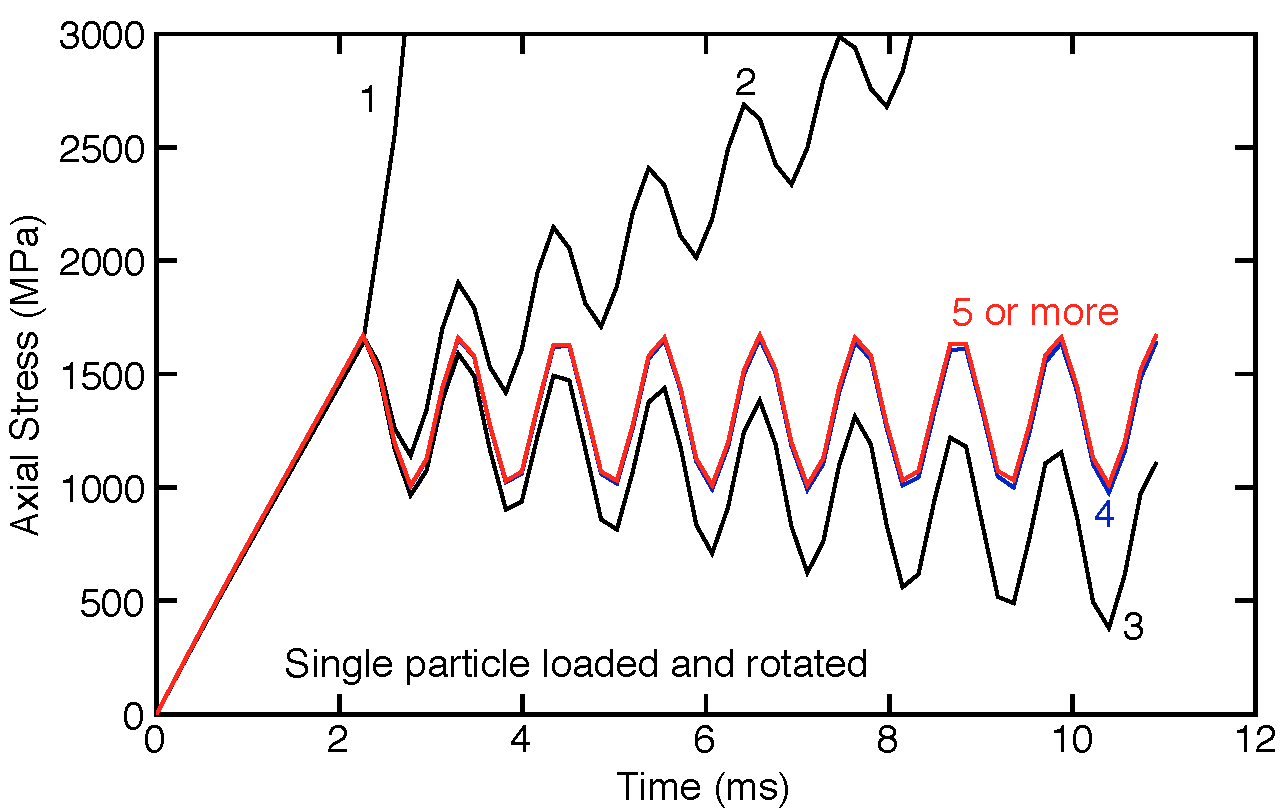
\includegraphics[width=5in]{IncrementalDef}
\caption{Calculation for a single particle loaded in tension, held, and then rotated. The different curves show $k_{max}$ or the number of terms used to expand the matrix exponential in the incremental deformation gradient.}
\label{dFCalc}
\end{center}
\end{figure}

\subsection{Mooney-Rivlin Material}

The Mooney-Rivilin material is an isotropic, elastic, hyperelastic material. It's stresses are based on a strain energy function that depends only on invariants to the left Cauchy-Green deformation tensor:
\begin{equation}
    \B = \F\F^T
\end{equation}
where $\F$ is the deformation tensor. The deformation tensor can be calculated by combining cumulative strain and rotation tensors (see {\tt HyperElastic.cpp} for the calculation). The strain energy is assumed to be
\begin{equation}
W = {G_1\over2}\left(\bar{I_1}-3\right) + {G_2\over2}\left(\bar{I_2}-3\right)^2 + {K\over2}\left(J-1\right)^2
\end{equation}
where $G_1$, $G_2$, and $K$ are material properties, $J=\det\F$, and the invariants are
\begin{eqnarray}
   \bar{I_1} & = & {B_{xx}+B_{yy}+B_{zz}\over J^{2/3}} \\
   \bar{I_2} & = & {1\over2}\left(\bar{I_1}^2 - {B_{xx}^2+B_{yy}^2+B_{zz}^2+2B_{xy}^2+2B_{xz}^2+2B_{yz}^2\over J^{5/3}}\right)
\end{eqnarray}
For low strains, this material is equivalent for a linear elastic, isotropic material with shear modulus $G_1+G_2$ and bulk modulus $K$. If $G_2=0$, the material is a neo-Hookean material. See below for an alternate compressibility terms. Some hyperelastic rubber models assume incompressible materials, which corresponds to $K\to\infty$; such models do not work in dynamic code (because wave speed is infinite).

To handle thermal and moisture strains, $\F$ is replaced by the deformation relative to the free expansion state:
\begin{equation}
     \F^* = {\F\over \lambda_{res}}
\end{equation}
where $\lambda_{res}$ is total extension due to free thermal and moisture expansion:
\begin{equation}
    1 + \alpha\Delta T + \beta \Delta c
\end{equation}
The total effect of expansion stress is included by replacing $J$ in all equations with $J/\lambda_{res}^3$.

The Cauchy (or true stress) is found by differentiating the strain energy to get
\begin{equation}
     \sigma = {G_1\over J^{5/3}}\left(\B - {I_1\over3}\I\right)
                     +  {G_2\over J^{7/3}}\left(I_1\B - \B^2 - {2I_2\over3}\I\right)   + K(J-1)\I
\end{equation}
where $I_1 = J^{2/3}\bar{I_1}$ and $I_2 = J^{4/3}\bar{I_2}$. The stress components explicitly evaluate to:
\begin{eqnarray}
      \s{xx} & = & K(J-1) + G_1{2B_{xx}-B_{yy}-B_{zz}\over 3J^{5/3}}   \nonumber\\
                  && \qquad\mbox{}    + G_2{B_{xx}(B_{yy}+B_{zz})-2B_{yy}B_{zz}-B_{xy}^2-B_{xz}^2+2B_{yz}^2\over 3J^{7/3} }\\
      \s{yy} & = & K(J-1) + G_1{2B_{yy}-B_{xx}-B_{zz}\over 3J^{5/3}}   \nonumber\\
                  && \qquad\mbox{}    + G_2{B_{yy}(B_{xx}+B_{zz})-2B_{xx}B_{zz}-B_{xy}^2+2B_{xz}^2-B_{yz}^2\over 3J^{7/3} }\\
      \s{zz} & = &  K(J-1) + G_1{2B_{zz}-B_{xx}-B_{yy}\over 3J^{5/3}}   \nonumber\\
                  && \qquad\mbox{}    + G_2{B_{zz}(B_{xx}+B_{yy})-2B_{xx}B_{yy}+2B_{xy}^2-B_{xz}^2-B_{yz}^2\over 3J^{7/3} }\\
       \t{xy} & = &  G_1{B_{xy}\over J^{5/3}} + G_2{B_{zz}B_{xy}-B_{xz}B_{yz}\over J^{7/3}}\\
       \t{xz} & = & G_1{B_{xz}\over J^{5/3}} + G_2{B_{yy}B_{xz}-B_{xy}B_{yz}\over J^{7/3}}\\
       \t{yz} & = & G_1{B_{yz}\over J^{5/3}} + G_2{B_{xx}B_{yz}-B_{xy}B_{xz}\over J^{7/3}}
\end{eqnarray}

\subsubsection{Plane Strain and Plane Stress Analysis}

For 2D analysis, $F_{xz}=F_{yz}=F_{zx}=F_{zy}=0$, which leads to zero for corresponding terms in $\B$. The resulting stresses are
\begin{eqnarray}
      \s{xx} & = & K(J-1) + G_1{2B_{xx}-B_{yy}-B_{zz}\over 3J^{5/3}}  
                    + G_2{B_{xx}(B_{yy}+B_{zz})-2B_{yy}B_{zz}-B_{xy}^2\over 3J^{7/3} }\\
      \s{yy} & = & K(J-1) + G_1{2B_{yy}-B_{xx}-B_{zz}\over 3J^{5/3}}   
                     + G_2{B_{yy}(B_{xx}+B_{zz})-2B_{xx}B_{zz}-B_{xy}^2\over 3J^{7/3} }\\
      \s{zz} & = &  K(J-1) + G_1{2B_{zz}-B_{xx}-B_{yy}\over 3J^{5/3}}   
                     + G_2{B_{zz}(B_{xx}+B_{yy})-2B_{xx}B_{yy}+2B_{xy}^2\over 3J^{7/3} }\\
       \t{xy} & = &  G_1{B_{xy}\over J^{5/3}} + G_2{B_{zz}B_{xy}\over J^{7/3}}\\
       \t{xz} & = & 0 \\
       \t{yz} & = & 0
\end{eqnarray}
For plane strain analysis $B_{zz}=1$. For plane stress analysis, one has to solve numerically for $B_{zz}$ to get $\s{zz}=0$ and then use that result to find $\e{zz}$ and other stresses.

\subsubsection{Alternate Bulk Modulus Term}

Two alternative compressibility terms (showing only that term) is

\begin{equation}
W = {K\over2}(\ln J)^2  \qquad{\rm and}\qquad W = {K\over2}\left({1\over2}(J^2-1) - \ln J\right)
\end{equation}

\noindent which gives normal Cauchy (or true stress) terms as
\begin{equation}
     \sigma = K {\ln J\over J}\I  \qquad{\rm and}\qquad \sigma = {K\over 2}\left(J-{1\over J}\right)\I
\end{equation}

\noindent Although these three compressibility terms show some significant differences when $J$ deviates significantly from 1, under most problems, $J$ will stay close to one. Two exceptions could be constrained compression or tension. Here, the only one that works well to very small or large $J$ is the second one above. This one correctly leads to inifinite positive stress as $J\to\infty$ and infinite negative stress as $J\to0$. This later one is the one currently implemented for this material in {\tt NairnMPM}.

\subsection{Ideal Gas Law}

The ideal gas material implements ideal gas law as a large deformation, hyperelastic material. It seems to work well for gas confined within a solid or constrained by rigid particles. It does not handle gas dynamics such as irreversible free expansion, but does handle reversible processes including coupled conversion of energy into heat ({\em i.e.}, cooling on expansion and heating on compression).

The ideal gas law is
\begin{equation}
    PV = nRT
\end{equation}
The ideal gas properties are defined by picking any reference pressure, $P_0$, reference temperature, $T_0$, and reference density, $\rho_0$. If $M$ is the molecular weight of the gas molecules, the reference density can be found from:
\begin{equation}
    \rho_0 = {P_0\over T_0} {M\over R}
\end{equation}
We can now eliminate $n$ and $R$ to derive
\begin{equation}
    P = P_0{V_0\over V}{T\over T_0} = P_0 {T\over T_0} {1\over J}
\end{equation}
where $J = \det \F = V/V_0$. The Cauchy stress due to this pressure is $-P\I$, which implies hyperelastic energy function determined from:
\begin{equation}
    \vec\sigma = - P_0 {T\over T_0} {1\over J}\I = {dU(J)\over dJ}\I
        \qquad{\rm or}\qquad
         U(J) = - P_i \ln J
\end{equation}
where $P_i = P_0T/T_0$ is the initial pressure (when $J=1$). This energy is equal to the energy per unit initial volume for isothermal compression or expansion of an ideal gas:
\begin{equation}
    U(J) = - {1\over V_0} \int_{V_0}^V P\thinspace dV = - {nRT\over V_0} \int_{V_0}^V {1\over V}\thinspace dV = - P_i \ln {V\over V_0} = - P_i \ln J
\end{equation}

For MPM calculations, the code needs a specific Kirchoff stress normalized to $\rho_0$ or
\begin{equation}
    \vec\tau^{(s)} = -{PJ\over \rho_0}\I  = - {P_0\over \rho_0} {T\over T_0}\I
\end{equation}
In coding, an incremental approach is preferred. 
If $\tau_n^{(s)}$ is any diagonal element of the specific Kirchoff stress tensor for time step $n$, then
\begin{equation}
   \tau_{n+1}^{(s)} = - {P_0\over \rho_0} {T_{n+1}\over T_0}  = - {P_0\over \rho_0} {T_n\over T_0} {T_{n+1}\over T_n}
       = \tau_n^{(s)} {T_{n+1}\over T_n}
\end{equation}
Note that the Kirchoff stress remains constant for isothermal expansion and compression.

The energy increment associated with this stress change is $dU = -P\thinspace dV$ work. The energy per unit mass using midpoint rule between initial and final pressure is therefore
\begin{equation}
    {dU\over \rho_0 V_0} = - {1\over2} {P_n+P_{n+1}\over \rho_0} 
         {V_{n+1} - V_n\over V_0} = - {1\over2} {P_n+P_{n+1}\over \rho_0} {V_{n+1}\over V_0}
         \left(1 - {V_n\over V_{n+1}}\right)
\end{equation}
Let deformation gradient for step $n+1$ be
\begin{equation}
       \F_{n+1} = \f\cdot\F_n  \quad{\rm where}\quad \f = \I + \Delta t\nabla\vec v
       \quad{\rm and}\quad J_{n+1} = \det \f J_n
\end{equation}
which leads to
\begin{equation}
    {dU\over \rho_0 V_0} = - {J_{n+1}\over2} {P_n+P_{n+1}\over \rho_0} 
         \left(1 - {1\over\det f}\right) = - {1\over2}
         \left({P_n\over \rho_{n}}\det f+{P_{n+1}\over \rho_{n+1}} \right)
         \left(1 - {1\over\det f}\right)
\end{equation}
But, $P/\rho$ is $-\tau^{(s)}$ leading to
\begin{equation}
    {dU\over \rho_0 V_0} =  {1\over2}
         \left(\tau_n^{(s)}\det f+\tau_{n+1}^{(s)} \right)
         \left(1 - {1\over\det f}\right)
\end{equation}
When conduction with energy coupling is activated, this entire energy is dissipated energy, which can lead to temperature changes.

When gas particles are present, they have to be initialized to the pressure (or stress) of
\begin{equation}
     \tau_i^{(s)} =  - {P_i\over \rho_0} = - {P_0\over \rho_0} {T\over T_0}
\end{equation}
where $T$ is the simulation reference temperature (need not be the gas reference temperature, which can be any desired reference condition). All simulations with gas particles must therefore specify a reference temperature in degrees Kelvin.

When doing conduction and energy coupling, this material needs head capacity and thermal conductivity. Heat capacity is calculated using ideal gas law theory (and any entered heat capacities will be ignored). Thermal conductivity, however, should be entered. The current code assumes conductivity is a temperature-independent property, although conductivity of a gas does vary with temperature. If simulations with large temperature changes of the gas are important, this material will need to be improved to allow temperature-dependent thermal conductivity.

\section{Two-State Isotropic Material}

The \code{BistableIsotropic} class inherits from \code{Isotropic}. It allows two different isotropic states and transitions  between the states based on various criteria. The two options are to have a jump to a new linear stress-strain curve (\code{DILATION\_RULE}) or to simply change the slope (\code{DISTORTION\_RULE} or \code{VONMISES\_RULE}). When jumping to a new curve (\code{DILATION\_RULE}), the deformed state can additionally define a new origin by adding an offset volumetric strain. The only new calculations needed are to change properties when a transition occurs and if there is a new stress-strain curve to calculate a jump in stresses to the new curve. The 3D stiffness equations with an offset volumetric strain for an isotropic material are
\begin{equation}
     \left(\begin{array}{c} \s{xx} \\ \s{yy} \\ \s{zz} \\ \t{xz} \\ \t{yz} \\ \t{xy} \end{array}\right)
       =  \left(\begin{array}{cccccc}
      C_{11} & C_{12} & C_{12} & 0 & 0 & 0 \\
      C_{12} & C_{11} & C_{12} & 0 & 0 & 0 \\
      C_{12} & C_{12} & C_{11} & 0 & 0 & 0 \\
      0 & 0 & 0 & C_{66} & 0 & 0 \\
      0 & 0 & 0 & 0 & C_{66} & 0  \\
      0 & 0 & 0 & 0 & 0 &  C_{66}  \end{array}\right)
     \left(\begin{array}{c} \e{xx} - {\Delta\over 3} -\er{}\\ \e{yy} - {\Delta\over 3} -\er{}\\ 
                   \e{zz} - {\Delta\over 3} - \er{}\\ 
                   \g{xz} \\ \g{yz} \\ \g{xy} \end{array}\right)
\end{equation}
where $\er{}=\a{}\DT+\b{}\Delta c$.
Whenever a change in state occurs in the \code{DILATION\_RULE}, these equations must be used to recalculate all components of stress.

\subsection{Plane Stress Equations}

The plane stress stiffness equations for in-plane stresses are
\begin{equation}
      \vvec{\s{xx}}{\s{yy}}{\t{xy}} = \symmat{Q_{xx}}{Q_{xy}}{0}{Q_{xx}}{0}{Q_{xyxy}}
          \vvec{\e{xx}- {\Delta\over 3}  - \er{}}{\e{yy}- {\Delta\over 3}  - \er{}}{\g{xx}}
 \end{equation}
with out-of-plane strain given  by
\begin{equation}
            \e{zz} = -{C_{12}\over C_{11}}(\e{xx}- {\Delta\over 3} -\er{}) - {C_{12}\over C_{11}}(\e{yy} - {\Delta\over 3}-\er{}) 
                   + {\Delta\over 3}  + \er{}
\end{equation}
For the super-class \code{Isotropic} material, the needed terms are stored as \code{mdm[1][1]} = \code{mdm[2][2]} $= Q_{xx}/\rho$,  \code{mdm[1][2]} $= Q_{xy}/\rho$,  \code{mdm[3][3]} $= Q_{xyxy}/\rho$,  \code{mdm[4][1]} =  \code{mdm[4][2]}$= -C_{12}/C_{11}$,  \code{me0[1]} = \code{me0[2]} = \code{me0[4]} = \code{CTE3}  $=\a{}$, \code{mc0[1]} = \code{mc0[2]} = \code{mc0[4]} = \code{CME3}  $=\b{}$, \code{mdm[1][3]} = \code{mdm[2][3]} = \code{me0[3]} =\code{mc0[3]} $=0$, and \code{normOffset} $=\Delta/3$.

\subsection{Plane Strain Equations}

The plane strain stiffness equations for in-plane stresses are
\begin{equation}
      \vvec{\s{xx}}{\s{yy}}{\t{xy}} = \symmat{C_{11}}{C_{12}}{0}{C_{11}}{0}{C_{66}}
          \vvec{\e{xx} - {\Delta\over 3}(1+\nu) - \err{}}{\e{yy} - {\Delta\over 3}(1+\nu)  - \err{}}{\g{xx}}
 \end{equation}
 where $\err{}=\a{}^{(r)}\DT+\b{}^{(r)}\Delta c$.
 In other words, a reduced offset and residual strains are needed. The out-of-plane stress is found from 3D equation and without reduced terms:
 \begin{equation}
            \s{zz} = C_{12}\left(\e{xx} - {\Delta\over 3} -\er{}\right) 
                            +C_{12}\left(\e{yy} - {\Delta\over 3} -\er{}\DT\right) 
                            -C_{11}\left({\Delta\over 3} +\er{}\right) 
\end{equation}
For the super-class \code{Isotropic} material, the needed terms are stored as \code{mdm[1][1]} = \code{mdm[2][2]} = \code{mdm[4][4]} $= C_{11}/\rho$,  \code{mdm[1][2]} $= C_{12}/\rho$,  \code{mdm[3][3]} $= C_{66}/\rho$,  \code{mdm[4][1]} =  \code{mdm[4][2]} $= C_{12}/\rho$, \code{me0[1]} = \code{me0[2]} $=\a{}(1+\v{})$, \code{mc0[1]} = \code{mc0[2]} $=\b{}(1+\v{})$, \code{me0[4]} = \code{CTE3} $=\a{}$, \code{mc0[4]} = \code{CME3} $=\b{}$, \code{me0[5]} = \code{me0[6]} $=\nu$, \code{mdm[1][3]} = \code{mdm[2][3]} = \code{mdm[4][3]} = \code{me0[3]} = \code{me0[7]} $=0$, \code{normOffset} $=\Delta/3$, and \code{nu} = $\v{}$.

\subsection{Special Cases for $E=0$}

If either $K$ or $G$ in any state is zero then the tensile modulus $E$ is also zero. Although this state is easy to derive in theory, in practice, it rarely gives useful results in dynamic MPM (except maybe as an inclusion in a composite material). A second problem is that it requires special cases to make it work with the super \code{Isotropic} class because that class has equations requiring $E\ne 0$. For these reasons, NairnMPM does not support zero modulus states in this material. It is easy to approximate such a state simply by setting $K$ and/or $G$ to a very small number.

\end{document}   